\documentclass[twocolumn]{class}


\addbibresource{References.bib}

% add path to images
\graphicspath{ {./images/} }

\title{Heart Disease Recognition \\ from heart beat audio signals}
\shorttitle{Heart Disease Prediction}

\github{https://github.com/DavideLigari01/advanced-biomedical-project}

\author{Ligari D. • Alberti A.}

\affil[1]{Department of Computer Engineering, Data Science, University of Pavia, Italy \newline\centering Course of Advanced Biomedical Machine Learning}

\keywords{ Heartbeat Classification • Machine Learning • Audio Features • Correlation Analysis • Ensamble Models}
\abstract{  
   Heart disease remains one of the leading causes of mortality worldwide, making early diagnosis crucial.
   This study aims to predict heart diseases by analyzing heartbeat audio signals using machine learning and network analysis. 
   We utilized a dataset from the PASCAL Classifying Heart Sounds Challenge 2011, which includes normal heart sounds, murmurs, extra heart sounds, extra systoles, and artifacts. 
   Various preprocessing techniques such as noise reduction, resampling, and segmentation were applied to ensure data quality.
   Features were extracted using methods like Mel-Frequency Cepstral Coefficients (MFCC), Chroma, RMS, ZCR, and spectral features. 
   Multiple machine learning models including LightGBM, XGBoost, CatBoost, Random Forest, and Multilayer Perceptron were trained and evaluated. 
   The best performing model achieved high accuracy in distinguishing between different heart sound categories. 
   This research highlights the potential of machine learning in cardiac diagnostics and provides a foundation for future advancements in the field.
   }
\firstauthor{Alberti Ligari}
\publicationdate{\today}


\begin{document}

\maketitle
\pagestyle{FirstPage}

\tableofcontents
% \nocite{dizdar_dns_2021}

% ------------------- START OF SECTIONS -------------------


% ------------------- Introduction -------------------

\section{Introduction}
\firstword{H}{eart} disease remains a leading cause of mortality worldwide, making early diagnosis critical for effective treatment and management. Traditional diagnostic methods are often invasive and expensive. Recent advancements in machine learning offer non-invasive alternatives using heart sound recordings. This paper explores the application of machine learning and network analysis to predict heart disease from heartbeat audio signals. The study addresses the challenges of data imbalance and noise in recordings by employing advanced data preprocessing techniques and robust machine learning models.

The dataset for this project, sourced from the PASCAL Classifying Heart Sounds Challenge 2011 (CHSC2011) and available on Kaggle, includes audio recordings of five types of heart sounds: Normal, Murmur, Extra Heart, Extrasystole, and Artifacts. The data was gathered from the general public via the iStethoscope Pro iPhone app and from clinical trials using the DigiScope digital stethoscope.

Preprocessing techniques such as noise reduction, resampling, and segmentation were applied to ensure data quality. Features were extracted using methods like Mel-Frequency Cepstral Coefficients (MFCC), Chroma, Root Mean Square (RMS), Zero-Crossing Rate (ZCR), and other spectral features. Various machine learning models, including LightGBM, XGBoost, CatBoost, Random Forest, and Multilayer Perceptron, were trained and evaluated. The best-performing model achieved high accuracy in distinguishing between different heart sound categories.

This research demonstrates the potential of machine learning in cardiac diagnostics and provides a foundation for future advancements in the field. By leveraging advanced techniques and comprehensive preprocessing, this study aims to enhance the accuracy of heart disease prediction, contributing to improved cardiovascular health outcomes.

\subsection{Problem Domain}

\subsection{Research Question}

\subsection{Previous Research}

\rowcolors{2}{blue!8}{blue!18}

\begin{table*}[ht!]
    \small
    \centering
    \begin{tabular}{|c|c|c|c|c|c|}
        \hline
        \textbf{Authors}                                                                & \textbf{Models}            & \textbf{Features}     & \textbf{Results} & \textbf{Anno} & \textbf{Dataset} \\ \hline
        W. Zhang et al \cite{Zhang_Han_Deng_2017}                                       & SVM                        & Spectrogram           & 0.76 Precision   & 2017          & N, M, EH, AR     \\ \hline
        SW. Deng et al \cite{Deng_Han_2016}                                             & SVM                        & DWT                   & 0.76 Precision   & 2016          & N, M, EH, AR     \\ \hline
        A. Raza et al \cite{Raza_Mehmood_Ullah_Ahmad_Choi_On_2019}                      & LSTM                       & 1D time series        & 0.80 Accuracy    & 2019          & N, M, ES         \\ \hline
        T. Alafif et al \cite{Alafif_Boulares_Barnawi_Alafif_Althobaiti_Alferaidi_2020} & 2D-CNN + transfer learning & MFCC                  & 0.89 Accuracy    & 2020          & N, A             \\ \hline
        Noman et al \cite{Noman_Ting_Salleh_Ombao_2019}                                 & Ensemble CNN               & 1D time series + MFCC & 0.89 Accuracy    & 2019          & N, A             \\ \hline
        Chen et al \cite{Chen_Ren_Hao_Hu_2018}                                          & 2D CNN                     & WT + Hilbert-Huang    & 0.93 Accuracy    & 2018          & N, M, ES         \\ \hline
        Our Model                                                                       & Ensemble Model (MLPs + RF) & MFCC + Chroma + ZCR   & 0.88 Accuracy    & 2024          & AR, M, N, EH, ES \\ \hline
    \end{tabular}
    \caption{Comparison of different models for classification. \textbf{Legend:} N: Normal, M: Murmur, EH: Extra Heartbeat, AR: Artifact, ES: Extra systoles, A: Abnormal}
\end{table*} % both
\pagestyle{OtherPage}

\section{Methods}
\subsection{Source of Data}
The dataset for this project was obtained from a Kaggle repository titled \textit{Dangerous Heartbeat Dataset (DHD)} \cite{Dangerous-Heartbeat-Dataset-DHD},
which in turn sources its data from the PASCAL Classifying Heart Sounds Challenge 2011 (CHSC2011) \cite{pascal-chsc-2011}.
This dataset comprises audio recordings of heartbeats, categorized into different types of heart sounds.
Specifically, the dataset consists of 5 types of recordings: Normal Heart Sounds, Murmur Sounds, Extra Heart Sounds, Extrasystole Sounds, and Artifacts.
Data has been gathered from the general public via the iStethoscope Pro iPhone app and from a clinic trial in hospitals using the digital stethoscope DigiScope.

\subsubsection*{Type of Sources} %Davide
The dataset comprises audio recordings collected from three distinct sources:
\paragraph{Type A:}
This subset includes recordings contributed by the general public through the iStethoscope Pro iPhone app.
Users from diverse backgrounds and locations have submitted these recordings, providing a wide range of heart sounds in various conditions.
\paragraph{Type B:}
This subset consists of recordings obtained from clinical trials conducted in hospitals using the DigiScope digital stethoscope.
These recordings are collected in controlled environments, contributing to a high-quality dataset for clinical applications.
\paragraph{Type C:}
This subset is a mixed collection that includes recordings from both the iStethoscope Pro app and the DigiScope digital stethoscope.
Additionally, this subset incorporates heart sound recordings sourced from various publicly available datasets on the internet.
This mixed dataset is valuable for its diversity and comprehensiveness, covering a broad spectrum of heart sound variations and abnormalities.

\noindent
These diverse sources ensure a robust dataset that supports comprehensive analysis and improves the generalizability of the heartbeat audio classification model.
\subsubsection*{Classes} % Davide

Heart sounds can be categorized into different classes based on their acoustic characteristics and clinical significance.
Accurate classification of these sounds is essential for diagnosing and treating a variety of cardiac conditions.
The primary categories include Normal heart sounds, Murmurs, Extra Heart Sounds, Artifacts, and Extra Systoles.
Understanding the distinct features and clinical implications of each class is a crucial step before building a
machine learning model to classify heartbeats.
This phase is particularly important for the identification of patterns that are characteristic of specific classes,
which in turn guides the selection of features to extract from the audio.
This knowledge aids in identifying specific patterns and anomalies within the heart sounds,
leading to more precise and reliable model predictions.

\paragraph{Normal}
The Normal category includes recordings of typical, healthy heart sounds. These sounds exhibit the characteristic ``lub-dub, lub-dub'' pattern,
where ``lub'' (S1) represents the closing of the atrioventricular valves and ``dub'' (S2) signifies the closing of the semilunar valves.
In a normal heart, the time interval between ``lub'' and ``dub'' is shorter than the interval from ``dub'' to the next ``lub,''
especially when the heart rate is below 140 beats per minute. Most normal heart rates at rest fall between 60 and 100 beats per minute,
though rates can vary from 40 to 140 beats per minute based on factors such as age and activity level.
Recordings may include background noises like traffic or radio sounds and may capture incidental noises such as breathing or microphone
contact with clothing or skin. It contains both clean and noisy normal recordings,
the latter featuring significant background noise or distortion, which simulates real-world conditions.\\
Figure \ref{fig:normal_heart_beat_audio} shows a sample of a normal heart beat audio.
The characteristic ``lub-dub, lub-dub'' pattern can be observed, where the peaks represent the ``lub'' (S1) and ``dub'' (S2) sounds of a healthy heart.

\begin{figure}[H]
    \centering
    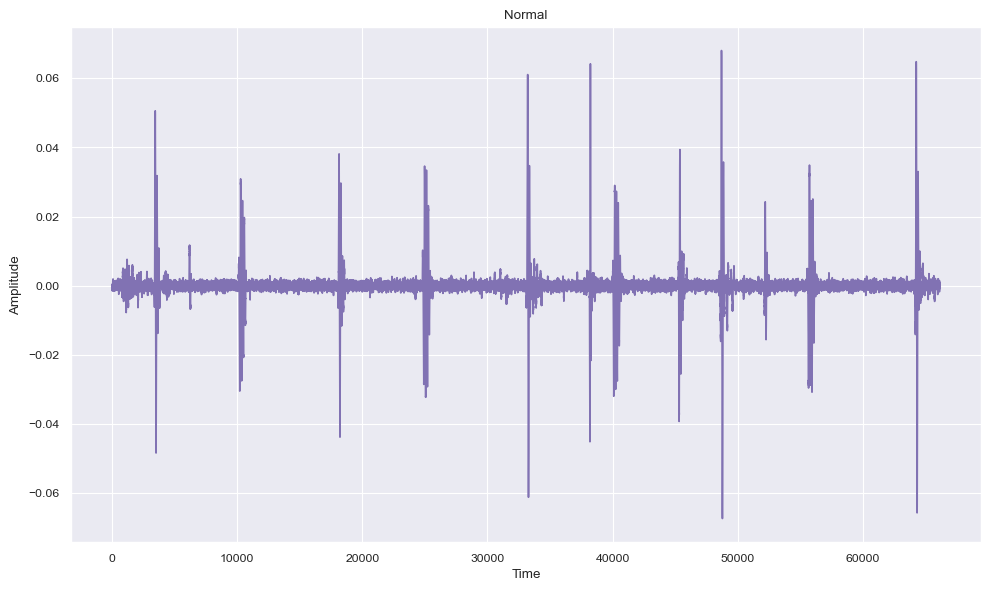
\includegraphics[width=.9\columnwidth]{../images/normal_heart_beat_audio.png}
    \caption{Sample of normal heart beat audio.}
    \label{fig:normal_heart_beat_audio}
\end{figure}

\paragraph{Murmur}
Heart murmurs are abnormal sounds during the heartbeat cycle, such as a ``whooshing, roaring, rumbling, or turbulent fluid'' noise, heard between
the ``lub'' and ``dub'' (systolic murmur) or between ``dub'' and ``lub'' (diastolic murmur).
These murmurs are typically indicative of turbulent blood flow in the heart and can signal various heart conditions, some of which may be serious.
It is crucial to distinguish murmurs from the normal ``lub-dub'' sounds since they occur between the primary heart sounds and not concurrently with them.
It also includes noisy murmur data, which mimics real-world recording scenarios by incorporating significant background noise and distortions.\\
Figure \ref{fig:murmur_heart_beat_audio} shows a sample of a murmur heart beat audio.
The presence of additional sounds between the ``lub'' and ``dub'' peaks can be observed, indicating the characteristic
``whooshing, roaring, rumbling, or turbulent fluid'' noise typical of heart murmurs.

\begin{figure}[H]
    \centering
    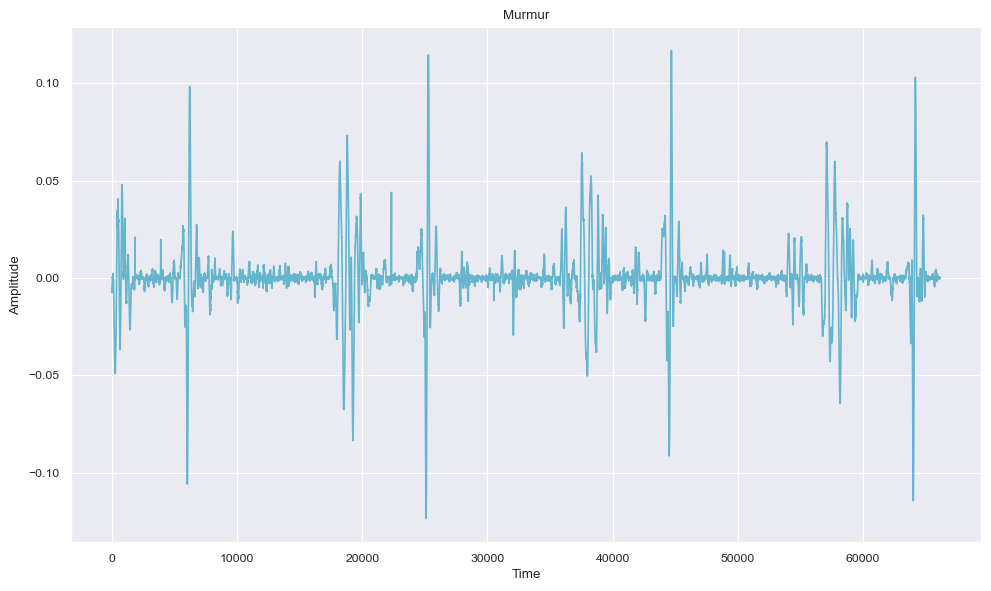
\includegraphics[width=.9\columnwidth]{../images/murmur_heart_beat_audio.png}
    \caption{Sample of murmur heart beat audio.}
    \label{fig:murmur_heart_beat_audio}
\end{figure}

\paragraph{Extra Heart Sound}
Extra heart sounds are characterized by an additional sound in the cardiac cycle, producing patterns such as ``lub-lub dub'' or ``lub dub-dub''.
These sounds can arise from physiological or pathological conditions. For example, a third heart sound (S3) may indicate heart failure or volume overload,
while a fourth heart sound (S4) can be associated with a stiff or hypertrophic ventricle.
Detecting these extra sounds is important for identifying potential heart diseases early, allowing for timely intervention and management.
Figure \ref{fig:extrahls_heart_beat_audio} shows a sample of an extra heart sound audio.
The presence of additional peaks within the normal ``lub-dub'' pattern indicates extra heart sounds, which can be
critical for diagnosing various heart conditions.

\begin{figure}[H]
    \centering
    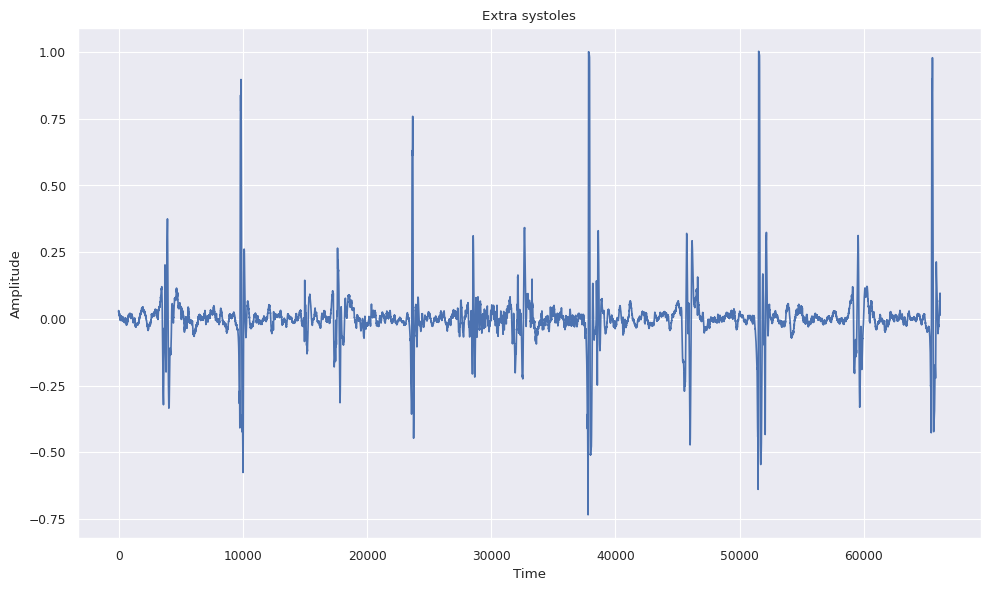
\includegraphics[width=.9\columnwidth]{../images/extrastoles_heart_beat_audio.png}
    \caption{Sample of extra heart sound audio.}
    \label{fig:extrahls_heart_beat_audio}
\end{figure}

\paragraph{Artifact}
The Artifact category consists of recordings with non-cardiac sounds, including feedback squeals, echoes, speech, music, and various types of noise.
These recordings generally lack discernible heart sounds and do not exhibit the temporal periodicity typical of heartbeats at frequencies below 195 Hz.
Accurately identifying artifacts is essential to avoid misinterpreting non-cardiac sounds as pathological heart sounds,
ensuring that data collection efforts focus on genuine heart sounds.
Figure \ref{fig:artifact_heart_beat_audio} shows a sample of an artifact heart beat audio, there can be observed that there is not a clear pattern in the audio.

\begin{figure}[H]
    \centering
    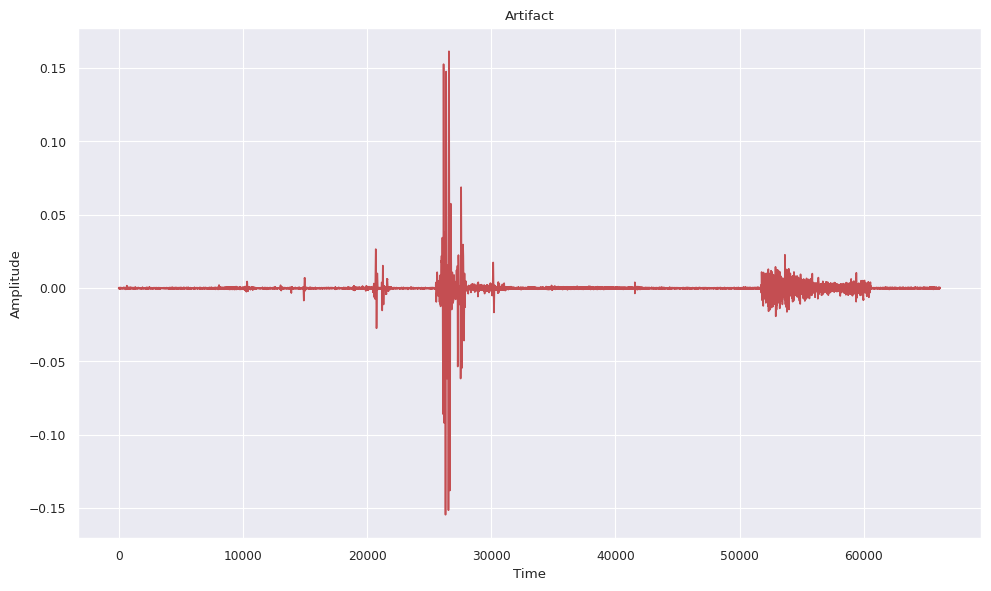
\includegraphics[width=.9\columnwidth]{../images/artifact_heart_beat_audio.png}
    \caption{Sample of artifact heart beat audio }\label{fig:artifact_heart_beat_audio}
\end{figure}

\paragraph{Extra systoles}
Extra systoles refers to extra or skipped heartbeats, resulting in irregular patterns such as ``lub-lub dub'' or ``lub dub-dub''.
Unlike the regular extra heart sounds, extra systoles are sporadic and do not follow a consistent rhythm.
These premature beats can occur in healthy individuals, particularly children, but they may also be associated with various heart diseases.
Identifying extra systoles is crucial as they can be early indicators of cardiac conditions that might require medical attention
if they occur frequently or in certain patterns.\\
In the audio signal depicted in Figure \ref{fig:extrastoles_heart_beat_audio}, irregularities within the normal “lub-dub” pattern are evident.
These irregularities manifest as additional peaks or skipped beats, indicating extra systoles.
\begin{figure}[H]
    \centering
    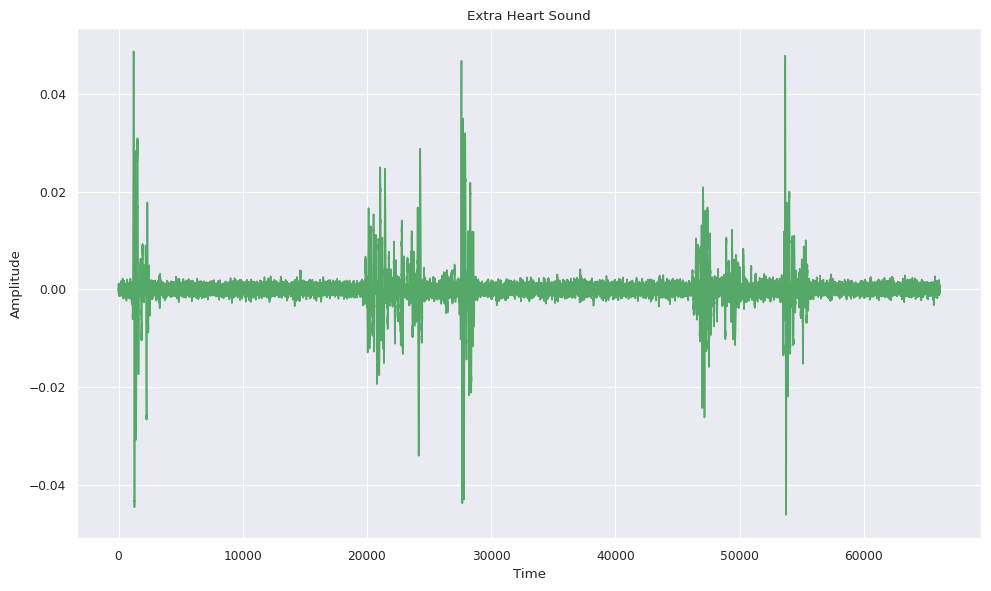
\includegraphics[width=.9\columnwidth]{../images/extrahls_heart_beat_audio.png}
    \caption{Sample of extra systoles heart beat audio }\label{fig:extrastoles_heart_beat_audio}
\end{figure}

\paragraph{Comparison of Heart Sounds}
In Figure \ref{fig:comparison_heart_beat_audio}, a comparison of the different classes of heart sounds can be observed.\\
As we can see, the “Artifact” signal appears erratic with no consistent pattern, likely representing noise or interference rather than true heart sounds.\\
The “Murmurs” signal shows irregular fluctuations in amplitude, which could indicate turbulent blood flow typically associated with murmurs. \\
The signal for “Extra Heart Beat Sound” has occasional spikes in amplitude that stand out from the baseline.\\
The “Normal” signal appears more uniform and regular compared to the others, reflecting the expected rhythm of a healthy heartbeat.
FInally, the signal for “Extra Systoles” shows extra spikes at irregular intervals,
indicating unexpected contractions of the heart muscle (systoles) occurring outside the normal rhythm.

\begin{figure}[H]
    \centering
    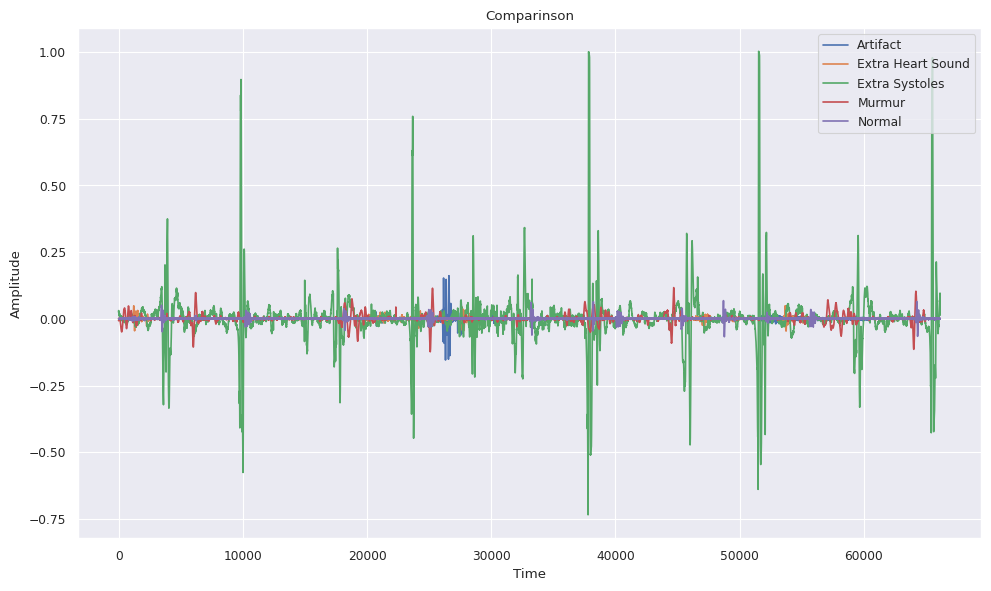
\includegraphics[width=.9\columnwidth]{../images/comparison_heart_beat_audio.png}
    \caption{Comparison of the different classes of heart sounds.}
    \label{fig:comparison_heart_beat_audio}
\end{figure}

\subsubsection*{Data Distribution} % Davide
Figure \ref{fig:DataExp_num_durations}, illustrates the significant class imbalance present in the dataset, particularly for the 'Extrastole' and 'Extrahls' classes,
which have far fewer samples compared to other classes.
This imbalance poses a challenge for the classification task,
as the model may struggle to learn and accurately predict the underrepresented classes due to the insufficient number of training examples.
To mitigate this issue, several strategies are employed.\\
Data augmentation techniques are applied to artificially increase the size of the dataset
by creating modified versions of the existing audio files through methods such as pitch shifting, time stretching, and adding noise.
Additionally, the original audio recordings are segmented into smaller clips, which not only increases the number of samples available for training but
also provides the model with more varied examples of heart sounds, enhancing its ability to generalize across different heart sound variations.\\
Furthermore, the effectiveness of oversampling and undersampling techniques is tested. Oversampling involves duplicating samples from the minority classes
to increase their representation in the training set, while undersampling involves reducing the number of samples from the majority classes
to balance the dataset. The data is split into training and testing sets with an 80\% - 20\% ratio, respectively.\\
A validation set is omitted due to the low number of samples available, ensuring that the maximum amount of data is used for training and testing the model.
\begin{figure}[H]
    \centering
    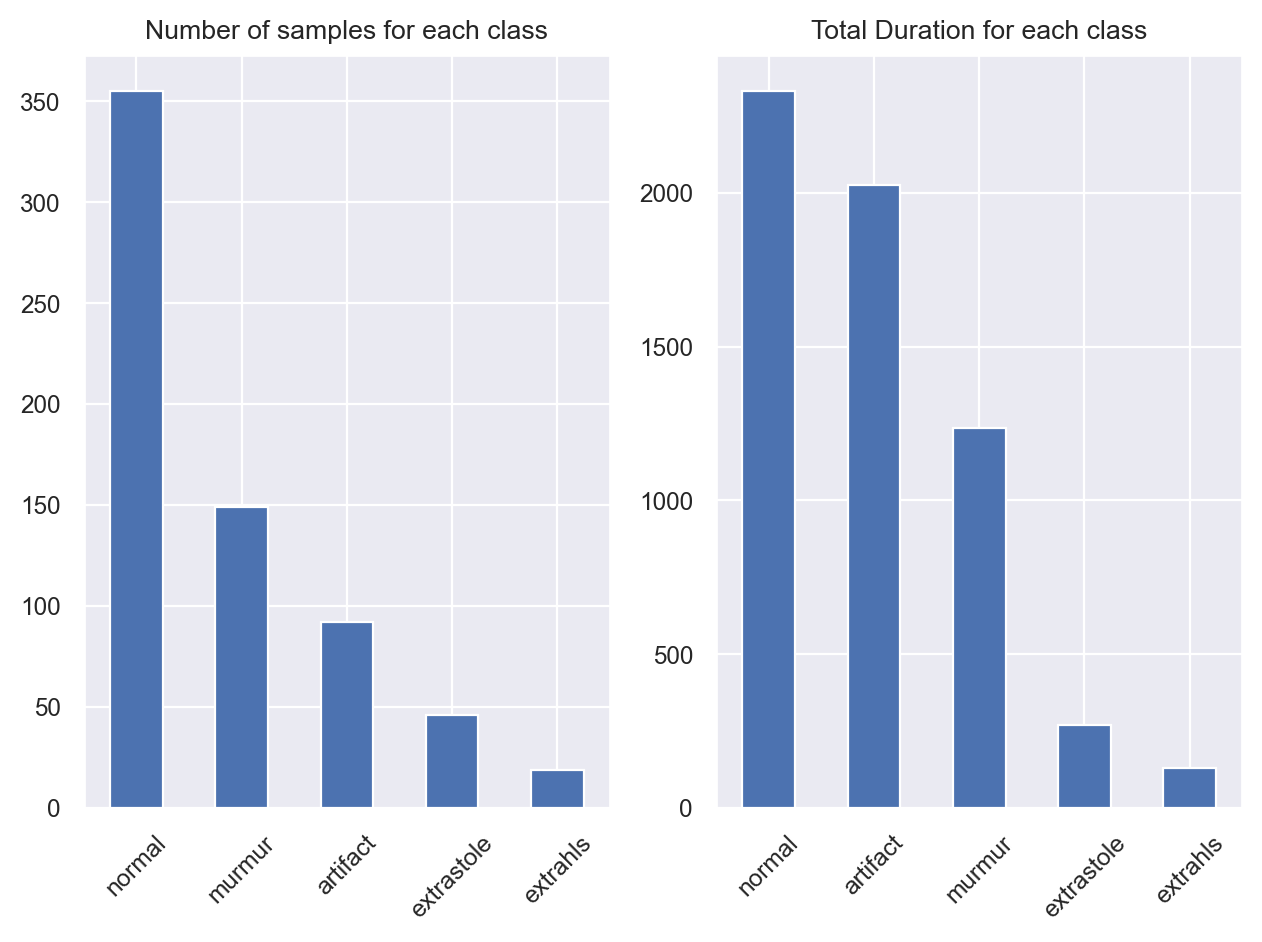
\includegraphics[width=1\columnwidth]{./images/DataExp_num_durations.png}
    \caption{Number of samples per duration.}
    \label{fig:DataExp_num_durations}
\end{figure}

 % mix

\subsection{Data Preprocessing}
To prepare the data several preprocessing operations were performed:

\vspace{0.2cm}\noindent
\textbf{Noise Reduction:} the audio data was already provided in a clipped format 
to minimize noise and irrelevant information.

\vspace{0.2cm}\noindent
\textbf{Normalization}: the audio are loaded using the \textit{torchaudio.load()} 
function, which normalized the audio signals in the range [-1, 1]. 

\vspace{0.2cm}\noindent
\textbf{Removal of Corrupted Files:} corrupted files were identified and removed 
from the dataset to ensure data quality.

\vspace{0.2cm}\noindent
\textbf{Outlier Detection and Removal:} we investigated the average duration of 
each class and found the 'artifact' class to have a significantly larger average 
duration. This was due to a few long lasting audio 
recordings (see Figure \ref{fig:DataExp_outliers_Artifacts}). A large number of samples from 
the same audio might not be as informative, thereby we used IQR to detect and remove outliers.

\vspace{0.2cm}\noindent
\textbf{Resampling:} we evaluated two sampling rates to determine the optimal rate 
for heartbeat sounds and all audio files were resampled to a common frequency of 4000 Hz 
(see Section \ref{sec:sampling_rate}).

\vspace{0.2cm}\noindent
\textbf{Segmentation:} the audio data was segmented into 1-second intervals, 
identified as the optimal extraction interval (see Section \ref{sec:extraction_interval}), as
it offered both good performance and dataset size increasing.

\vspace{0.2cm}\noindent
\textbf{Hop and Window Size}: the hop size determines the number of samples between 
successive windows, while the window size determines the number of samples considered. 
Each feature was extracted using the same window length and hop length facilitating a 
fair assessment of each feature's contribution to the classification task. 

\begin{figure}[H]
	\centering
	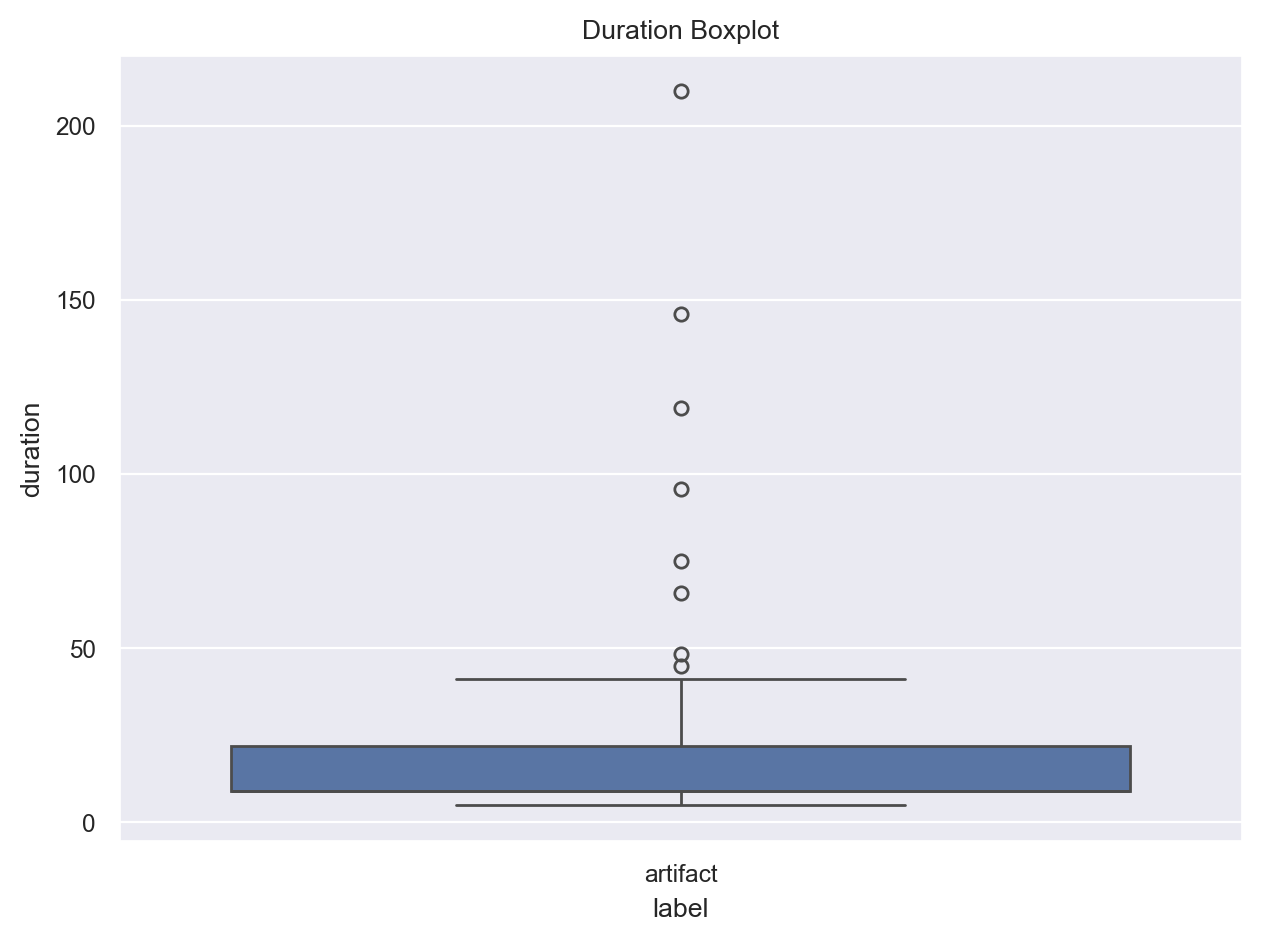
\includegraphics[width=1\columnwidth]{./images/DataExp_outliers_artifact.png}
	\caption{Outliers in the Artifacts class.}
	\label{fig:DataExp_outliers_Artifacts}
 \end{figure}\subsection{Data Preprocessing}
 % Andrea

\subsection{Feature Extraction}
s demonstrated by \cite{Raza_Mehmood_Ullah_Ahmad_Choi_On_2019} and \cite{Chen_Sun_Chen_Xie_Wu_Xu_2021}, MFCCs 
are highly effective features for heartbeat classification. In addition to MFCCs, 
we incorporated other features to capture various characteristics of heart sounds, enhancing the classification accuracy.
The features used are explained in the following section.

\subsubsection{Features Type}  % Andrea
\textbf{MFCC}\newline
Mel-Frequency Cepstral Coefficients (MFCCs) are representations of the short-term power spectrum of sound. 
They are derived by taking the Fourier transform of a signal, mapping the powers of the spectrum onto the mel 
scale, taking the logarithm, and then performing a discrete cosine transform. MFCCs are effective in capturing 
the timbral texture of audio and are widely used in speech and audio processing due to 
their ability to represent the envelope of the time power spectrum.
In heartbeat classification, MFFCs can reflect the different perceived quality of heart sounds,
such as the presence of murmurs or other anomalies.

\vspace{0.3cm}\noindent
\textbf{Chroma STFT}\newline
Chroma features represent the 12 different pitch classes of music (e.g., C, C\#, D, etc.). 
They are particularly useful for capturing harmonic and melodic characteristics in music. 
By mapping audio signals onto the chroma scale, these features can identify pitches regardless 
of the octave, making them useful for analyzing harmonic content in heart sounds.

\vspace{0.3cm}\noindent
\textbf{RMS}\newline
Root Mean Square (RMS) measures the magnitude of varying quantities, in this case, 
the amplitude of an audio signal. It is a straightforward way to compute the energy of 
the signal over a given time frame. RMS is useful in audio analysis for detecting volume 
changes and can help identify different types of heartbeats based on their energy levels.
For example, in a given timeframe the RMS may be altered by the presence of a murmur
with respect to a normal heart sound.

\vspace{0.3cm}\noindent
\textbf{ZCR}\newline
Zero-Crossing Rate (ZCR) is the rate at which a signal changes sign, indicating how often the signal 
crosses the zero amplitude line. It is particularly useful for detecting the noisiness and the temporal 
structure of the signal. In heartbeat classification, ZCR can help differentiate between normal and abnormal 
sounds by highlighting changes in signal periodicity.

\vspace{0.3cm}\noindent
\textbf{CQT}\newline
Constant-Q Transform (CQT) is a time-frequency representation with a logarithmic frequency scale, making it 
suitable for musical applications. Since it captures more detail at lower frequencies, it may be useful for analyzing 
the low-frequency components of heart sounds.

\vspace{0.3cm}\noindent
\textbf{Spectral Centroid}\newline
The spectral centroid indicates the center of mass of the spectrum and is often perceived as the brightness of a 
sound. It is calculated as the weighted mean of the frequencies present in the signal, with their magnitudes as 
weights. In heart sound analysis, a higher spectral centroid can indicate sharper, more pronounced sounds, 
while a lower centroid suggests smoother sounds. 

\vspace{0.3cm}\noindent
\textbf{Spectral Bandwidth}\newline
Spectral bandwidth measures the width of the spectrum around the centroid, providing an indication of the range 
of frequencies present. It is calculated as the square root of the variance of the spectrum. This feature helps 
in understanding the spread of the frequency components in the heart sounds, which can be indicative of different 
heart conditions.

\vspace{0.3cm}\noindent
\textbf{Spectral Roll-off}
Spectral roll-off is the frequency below which a certain percentage of the total spectral energy lies. It is 
typically set at 85\% and helps distinguish between harmonic and non-harmonic content. In heartbeat classification, 
spectral roll-off can be used to differentiate between sounds with a concentrated energy distribution and those with more dispersed energy.
\subsubsection{Sampling Rate Selection} % Andrea
\label{sec:sampling_rate}
The sampling rate of the data were heterogeneous, ranging from 4000 Hz to 44100 Hz, with a majority of the data being sampled at 4000 Hz.
To assess the impact of the sampling rate on the classification performance, we trained different models on
different features, extracted at different sampling rates and from various intervals. Each model is then 
evaluated using different metrics, taking into account the class imbalance issue.
We also consider a possible dependency between the sampling rate and the extraction interval, as shown 
in Algorithm \ref{alg:sr_choice}.

\begin{algorithm}
    \small
    \caption{Sampling rate choice}
    \label{alg:sr_choice}
    \begin{algorithmic}[1]
    \State \textbf{Input:}
    \State {features} = [\texttt{mfcc30 \& 120}, \texttt{cqt30 \& 70}, \texttt{chroma12}]
    \State {sampling\_rates} = [\texttt{mix}, \texttt{4000}]
    \State {extraction\_intervals} = [\texttt{0.5}, \texttt{1}, \texttt{2}, \texttt{3}]
    \State {models} = [\texttt{rf}, \texttt{svm-rbf}, \texttt{lr}]
    \State {metrics} = [\texttt{macrof1}, \texttt{mcc}]
    
    \vspace{0.2cm}
    \For{sr \textbf{in} sampling\_rates}
        \For{interval \textbf{in} extraction\_intervals}
            \For{feature \textbf{in} features}
                \State \textbf{extract} {feature} with {interval} at {sr}
                \For{model \textbf{in} models}
                    \State \textbf{train} {model} with extracted {feature}
                    \For{metric \textbf{in} metrics}
                        \State \textbf{evaluate} {model} with {metric}
                    \EndFor
                \EndFor 
            \EndFor
        \EndFor
    \EndFor
    
    \State \textbf{Output:}
    \State Given all the results, group by \texttt{model} and average the values of a specific \texttt{metric} across \texttt{features}
    
    \end{algorithmic}
    \end{algorithm}

    \noindent
The results, reported in Figure \ref{fig:FE_sampling_rate.png} showed no evident advantage to using a mix of sampling frequencies over a fixed resampled sample rate. 
Moreover, employing a fixed sample rate of 4000 Hz reduces the risk of introducing bias, enhances efficiency, 
and permits the use of a broader range of features and models.

\begin{figure}[H]
    \centering
    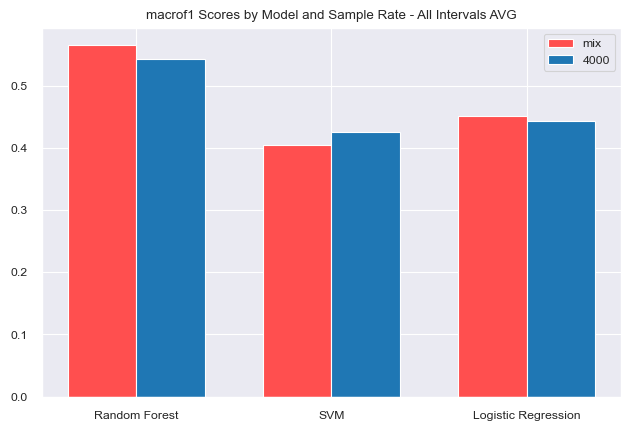
\includegraphics[width=1\columnwidth]{./images/FE_sampling_rate.png}
    \caption{Comparison of the macro F1 score for different sampling rates.}
    \label{fig:FE_sampling_rate.png}
\end{figure}


\subsubsection{Extraction Interval Selection}  % Andrea
\label{sec:extraction_interval}
The choice of the extraction interval 

\subsubsection{Number of Features per Type} % Davide % mix

\subsection{Feature Selection}
Given the large number of features (338 in total), it was necessary to identify and remove features that are poorly correlated with
the target variable as well as those that are highly correlated with each other. Due to the high number of features, a visual approach,
such as a correlation matrix, was not feasible. Instead, two filters were applied to select the most
relevant features using the Spearman correlation coefficient, as the normality test failed.\\
The first filter is based on the correlation between the features and the target variable. Features with a correlation below a certain
threshold with the target variable are removed.\\
The second filter focuses on the correlation among the features themselves.
It counts, for each feature, the number of other features with which it has a correlation above a certain threshold. Features with a
number of correlations above a specified threshold are then removed.\\

\begin{algorithm}
    \caption{Feature Selection Process}
    \begin{algorithmic}[1]
        \State \textbf{Step 1:} Compute  the normal test (D'Agostino Pearson).
        \State \textbf{Step 2:} Compute the Spearman correlation coefficient for each feature with the target variable.
        \State \textbf{Step 3:} Apply the first filter to remove features with a correlation below a certain threshold with the target variable.
        \State \textbf{Step 4:} Compute the correlation matrix among all features.
        \State \textbf{Step 5:} Apply the second filter to remove features that have a high number of correlations (above a certain threshold)
        with other features.
        \State \textbf{Step 6:} Choose threshold values empirically and apply the filters using various combinations of these thresholds.
        \State \textbf{Step 7:} Train Random Forest models on the filtered data to evaluate performance and select the best combination of thresholds.
    \end{algorithmic}
\end{algorithm}

\subsubsection*{Threshold Selection and Model Evaluation}

Threshold values were chosen empirically and the filters were applied using the combinations shown in Table \ref{tab:threshold_values}.
Using the filtered data, Random Forest models were trained and evaluated, as Random Forest was found to be the best performing model.
The optimal combination of thresholds was found to be: threshold 1 = 0, threshold 2 = 0.6 and number of features = 30, resulting in 30 features.

\rowcolors{2}{blue!8}{blue!18}
\begin{table}[h]
    \centering
    \small
    \begin{tabular}{|c|c|c|}
        \hline
        \textbf{Threshold} & \textbf{Values}                 \\
        THRESHOLD 1        & 0 - 0.1 - 0.2 - 0.3 - 0.4 - 0.5 \\
        THRESHOLD 2        & 0.6 - 0.7 - 0.8 - 0.9 - 1       \\
        N° FEATURES        & 5 - 10 - 15 - 20 - 25 - 30 - 40 \\
        \hline
    \end{tabular}
    \caption{threshold values}
    \label{tab:threshold_values}
\end{table}
\noindent
With threshold 1 = 0, the filter on the correlation between the features and the target variable was effectively bypassed.
However, with threshold 2 = 0.6, a stringent filter was applied on the correlation among the features themselves,
removing features that had a correlation above 0.6 with at least 30 other features. This indicates that having features
highly correlated with each other is more detrimental to the model than having features poorly correlated with the target variable.\\
Figure \ref{fig:comparison_model_on_all_features_vs_model_on_best} shows the results obtained with the model trained on filtered features
compared to the model trained on all features. As demonstrated, the model trained on filtered features performs significantly better.

\begin{figure}[H]
    \centering
    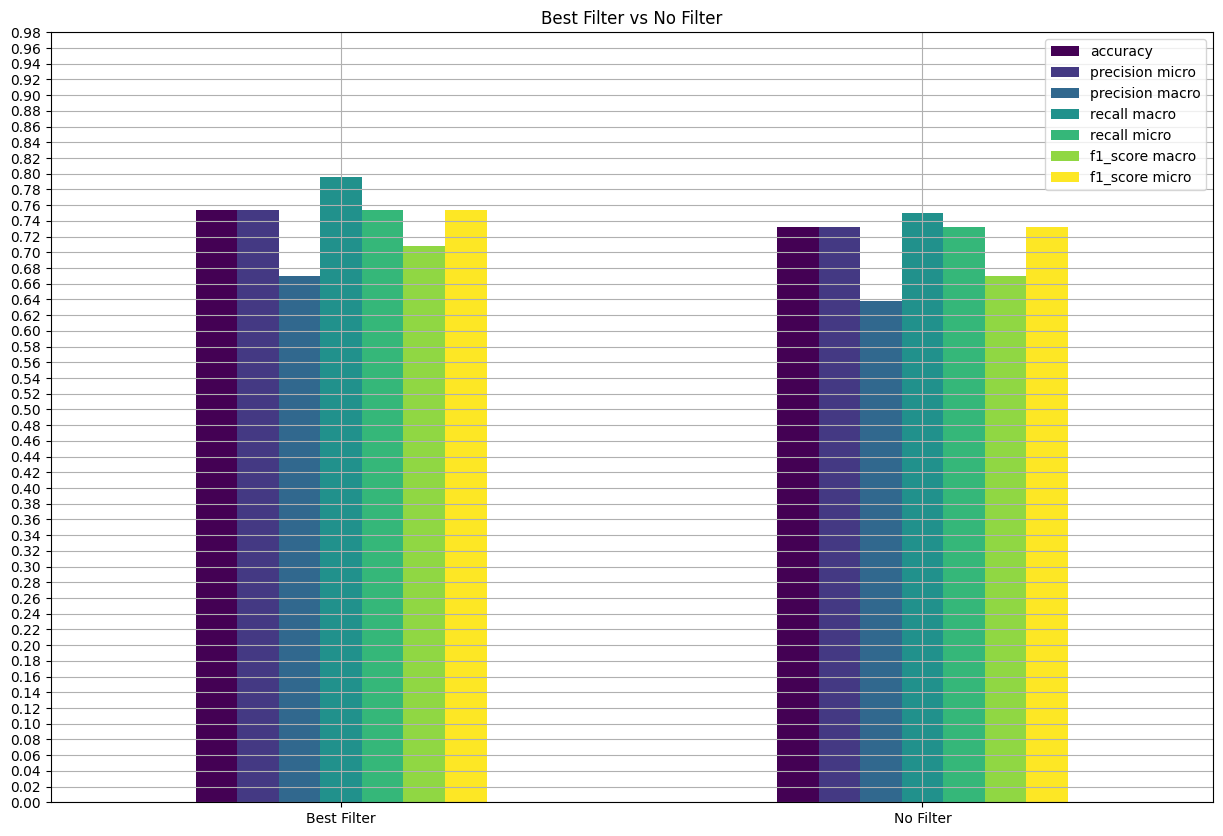
\includegraphics[width=0.9\columnwidth]{../images/model_on_all_features_vs_model_on_best.png}
    \caption{Comparison of different metrics between the model on all features and the model on the filtered ones}
    \label{fig:comparison_model_on_all_features_vs_model_on_best}
\end{figure}

\subsubsection*{Selected Features and Correlation Matrix}

From this analysis, 41 features remained: 28 MFCC, 12 Chroma, and 1 ZCR.
The correlation matrix of the filtered features is shown in Figure \ref{fig:correlation_matrix}.
This matrix illustrates the pairwise correlation between the selected features, with the color intensity
indicating the strength and direction of the correlation. Dark red cells represent high positive correlations,
while dark blue cells indicate high negative correlations.

\begin{figure}[H]
    \centering
    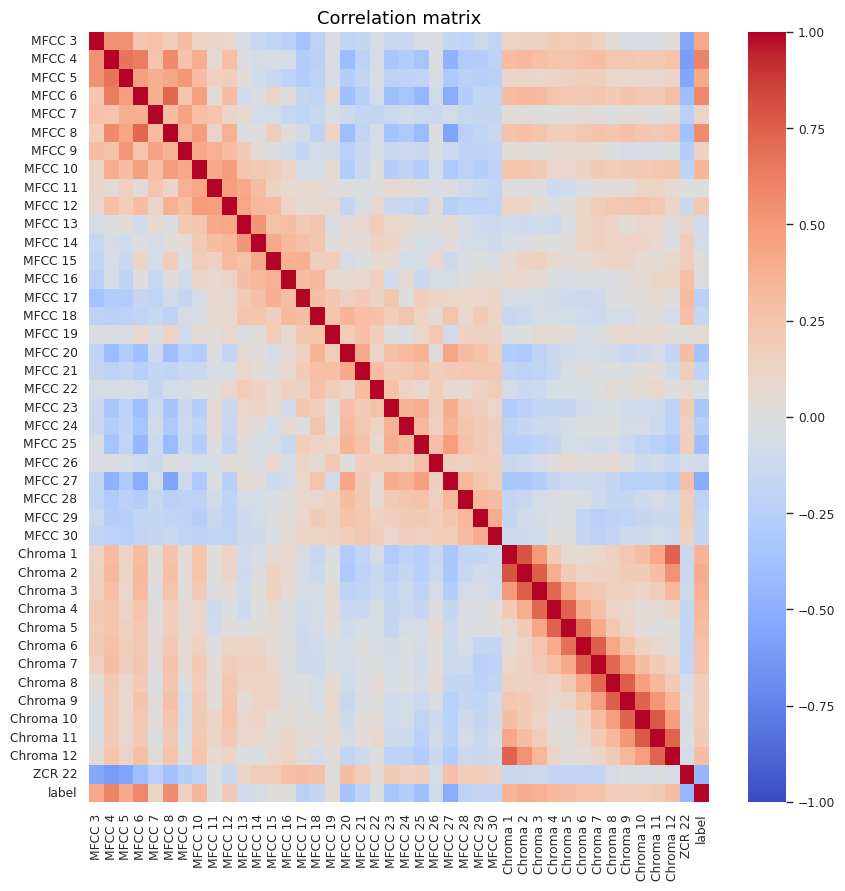
\includegraphics[width=0.9\columnwidth]{../images/correlation_matrix.png}
    \caption{Correlation matrix of the filtered features}
    \label{fig:correlation_matrix}
\end{figure}
\noindent
The matrix demonstrates that the remaining features have low correlations with each other, as evidenced by the predominantly
light colors away from the diagonal. This implies that the features are relatively uncorrelated, preventing multicollinearity
issues and enhancing the robustness of the model. The high diagonal values indicate that each feature is perfectly correlated
with itself, which is expected. However, the off-diagonal values being close to zero for most feature pairs confirm that the filtering
process was effective in selecting features that do not exhibit high inter-correlations.


 % Davide

\subsection{Models} % Davide

\subsubsection*{Metrics}

In this project, various metrics evaluate the heartbeat audio classification model, focusing on multiclass classification with imbalanced classes.

\paragraph{Accuracy}
Accuracy measures the ratio of correct predictions to the total number of predictions:
\[
    \text{Accuracy} = \frac{\text{Correct Predictions}}{\text{Total Predictions}}
\]
It is straightforward but can be misleading with imbalanced classes.

\paragraph{Balanced Accuracy}
Balanced accuracy addresses class imbalance by averaging recall across classes:
\[
    \text{Balanced Accuracy} = \frac{1}{N} \sum_{i=1}^{N} \frac{TP_i}{TP_i + FN_i}
\]
where \(N\) is the number of classes, \(TP_i\) is true positives, and \(FN_i\) is false negatives for class \(i\).

\paragraph{Matthews Correlation Coefficient (MCC)}
MCC evaluates performance by considering all classes:

\[
    \text{MCC} = \frac{\sum_k \sum_l \sum_m C_{kk} C_{lm} - C_{kl} C_{mk}}{\sqrt{\sum_k \left( \sum_l C_{kl} \right) \left( \sum_{k' \ne k} \sum_{l'} C_{k'l'} \right)} \sqrt{\sum_k \left( \sum_l C_{lk} \right) \left( \sum_{k' \ne k} \sum_{l'} C_{l'k'} \right)}}
\]
This comprehensive metric accounts for true and false predictions, making it robust for imbalanced datasets.

\paragraph{Precision and Recall}
Precision measures the accuracy of positive predictions:
\[
    \text{Precision} = \frac{TP}{TP + FP}
\]
Recall measures the proportion of actual positives correctly identified:
\[
    \text{Recall} = \frac{TP}{TP + FN}
\]
Micro variants aggregate these metrics across all classes, while macro variants average them per class, 
offering insights into individual class performance.

\paragraph{F1 Score}
The F1 score balances precision and recall:
\[
    \text{F1 Score} = 2 \times \frac{\text{Precision} \times \text{Recall}}{\text{Precision} + \text{Recall}}
\]
Micro and macro variants provide overall and class-specific performance evaluations, respectively.

\paragraph{ROC Curve and AUC}
For binary classification, the ROC curve plots true positive rate against false positive rate, and AUC summarizes the model's discriminatory ability,
 with higher AUC indicating better performance.

\paragraph{Risk Score}
The risk score evaluates the model's ability to avoid misclassifying heart disease as normal:
\[
    \text{Risk score} = \frac{FP}{FP + TP}
\]
A lower risk score indicates better performance. Disease-specific risk scores can provide detailed insights into different heart conditions. % Davide

\subsubsection{Prevention Model}
The goal of the prevention model is to provide an accessible tool for the early diagnosis of heart 
diseases, potentially usable by non-experts. Therefore, it is crucial to develop a model that 
minimizes the number of false normal predictions to accurately indicate the presence or not
of disease or identify artifacts in the provided data.

To achieve this, different heart diseases were grouped together, transforming the problem 
into a 3-class classification task: normal, disease, and artifact. Grouping the diseases not 
only simplified the classification but also balanced the class distribution. The data was 
divided into training and testing sets in an 80-20 ratio, and various models were evaluated, 
as shown in Table \ref{tab:models}.

The primary metrics for evaluating the models were the ROC-AUC score, false positive rate (FPR), 
and true positive rate (TPR), with F1-score and accuracy as secondary metrics. 
To adapt binary metrics for multi-class classification, the one-vs-rest strategy was employed. 
Specifically, we focused on the normal-vs-rest case to minimize false normal predictions.

In summary, each model was trained on the 3-class classification problem but was evaluated based on 
its binary classification performance (normal-vs-rest). The best model was selected based on its 
ROC-AUC score and performance at specific FPR levels (1\%, 5\%, 10\%, and 20\%). The objective was 
to minimize false normal predictions while maximizing true normals. A model predicting no cases 
as normal to achieve a 0\% FPR would be ineffective. % Andrea

\subsubsection*{Support Model}
In addition to the Prevention model, we developed a complementary model designed to assist clinicians in diagnosing heart diseases.
This model aims to accurately classify all classes present in the dataset, avoiding any simplifications, to ensure comprehensive diagnostic support.\\
Given the highly imbalanced nature of the dataset, where certain classes contain significantly fewer samples, traditional accuracy metrics can be misleading.
To address this, we explored various balancing techniques, but they did not yield satisfactory results.
Consequently, we prioritized metrics that provide equal importance to all classes, including the macro F1-score, balanced accuracy,
and Matthews Correlation Coefficient (MCC). These metrics collectively offer a robust evaluation by accounting for class imbalance,
ensuring that minority classes receive adequate consideration alongside majority classes.\\
A particular emphasis was placed on the 'Normal' class, focusing on minimizing false positives. This is crucial for patient safety,
as misclassifying abnormal heart sounds as normal could lead to missed diagnoses and delayed treatment.
To address this concern, we introduced a 'Risk score' that quantifies the impact of normal false positives, allowing
the model to be more sensitive to this critical aspect. This score was further adapted to evaluate individual diseases,
enhancing our ability to assess the model's risk for each specific condition.\\
The selection of the best model was guided by the macro F1-score and balanced accuracy.
These metrics comprehensively reflect performance across all classes, ensuring that no disease category is overlooked.
After identifying the optimal model, we employed explainability techniques to elucidate the model’s decision-making process.
This step is crucial because the model's outputs directly impact patient care; therefore, transparency and interpretability are essential.
By providing clinicians with insights into how the model arrives at its conclusions, we enhance trust and facilitate informed clinical decisions.\\
To achieve this, we computed feature importance using Permutation Feature Importance, which, according to A. Fisher et al.\cite{fisher2019modelswrongusefullearning},
highlights the most influential factors driving the model's predictions.\\
Additionally, we applied SHAP (SHapley Additive exPlanations) values, introduced by Scott M. Lundberg and
Su{-}In Lee \cite{DBLP:journals/corr/LundbergL17}, to interpret the model's output at the individual prediction level.
SHAP values provide a detailed breakdown of each prediction, illustrating the impact of specific features on the model's decision.
Based on the SHAP values, we identified the areas in the audio signal that significantly influenced the model's classification.\\
By integrating these explainability techniques, we ensure that the model’s decision-making process is transparent and comprehensible.
This not only builds confidence among clinicians but also ensures that the model's outputs are actionable and reliable in a clinical setting. % Davide

\subsubsection{Experimented Architectures}
\rowcolors{2}{blue!8}{blue!18}
\begin{table}[ht!]
    \centering
    \footnotesize
    \begin{tabular}{|l|l|}
        \hline
        \textbf{Name}           & \textbf{Architecture (hidden layers)}                                 \\ \hline
        Random Forest                 & -                                                     \\ \hline
        XGBoost                 & -                                                     \\ \hline
        CatBoost                & -                                                     \\ \hline
        LightGBM                & -                                                     \\ \hline
        MLP\_Basic              & (128, 64, 32)                                         \\ \hline
        MLP\_Ultra              & (512, 256, 128, 64, 32)                               \\ \hline
        MLP\_Large              & (256, 128, 64, 32)                                    \\ \hline
        MLP\_Small              & (64, 32)                                              \\ \hline
        MLP\_Tiny               & (32, 16)                                              \\ \hline
        MLP\_Reverse            & (32, 64, 128, 256, 512, 256, 128, 64, 32)             \\ \hline
        MLP\_Bottleneck         & (512, 64, 32)                                         \\ \hline
        MLP\_Rollercoaster      & (512, 128, 256, 128, 256, 64, 32)                     \\ \hline
        MLP\_Hourglass          & (512, 256, 128, 64, 32, 64, 128, 256, 512)            \\ \hline
        MLP\_Pyramid            & (1024, 512, 256, 128, 128, 128, 64, 32)               \\ \hline
        MLP\_Wide               & (1024, 1024)                                          \\ \hline
        MLP\_WideUltra          & (1024, 1024, 128, 32)                                 \\ \hline
        MLP\_Sparse             & (32, 16, 8)                                           \\ \hline
        MLP\_Dropout            & (128, 64, 32)                                         \\ \hline
        MLP\_Ensemble1          & MLP\_Basic, Large, Ultra                    \\ \hline
        MLP\_Ensemble2          & RandomForest, MLP\_Ultra                              \\ \hline
        MLP\_Ensemble3          & MLP\_Rollercoaster, Large                        \\ \hline
        MLP\_Ensemble4          & MLP\_Rollercoaster, Large, Ultra            \\ \hline
        MLP\_Ensemble5          & RandomForest, MLP\_Ultra, Rollercoaster          \\ \hline
        MLP\_Ensemble6          & MLP\_Rollercoaster, Large, Ultra, Wide \\ \hline
        ALL\_Ensemble           & All models majority vote                              \\ \hline
        CB\_ALL\_Ensemble       & All models CatBoost                                   \\ \hline
    \end{tabular}
    \caption{Models names and architectures.}
    \label{tab:models}
\end{table}

The architectures of the models used in the experiments are detailed in Table \ref{tab:models}. 
Special attention is given to the ensemble models, which combine predictions from multiple models 
to enhance overall performance.\\
\noindent
All MLP\_Ensemble models consist of the individual models listed in their architecture name. 
These models’ predictions are combined using a soft voting strategy, where the final prediction is 
determined by the argmax of the sum of the predicted probabilities from each model. This approach is 
effective when the models are well-calibrated and exhibit complementary strengths and weaknesses.\\
\noindent
The ALL\_Ensemble model aggregates the predictions of all individual models using a majority vote strategy. 
In contrast, the CB\_ALL\_Ensemble model also considers all individual models but uses a CatBoost model to 
aggregate the predictions. This allows for a more flexible voting strategy, potentially leading to improved 
performance. % Andrea


\subsection{Tools and Software}

This study utilized several powerful libraries and tools for data processing, model training, and evaluation:

\begin{itemize}[leftmargin=*]
    \item \textbf{Scikit-learn}: Used for MLP, RF, and metrics such as F1, Balanced Accuracy, Accuracy, MCC, ROC, AUC, permutation importance, train-test split, confusion matrix and voting classifiers.
    \item \textbf{Torchaudio}: Used to load the audio, for MFCC extraction and audio resampling.
    \item \textbf{Librosa}: Used for other features extraction and audio processing and augmentation.
    \item \textbf{Imblearn}: Applied for handling imbalanced datasets with techniques such as undersampling, oversampling, and SMOTEN.
    \item \textbf{Numpy}: Essential for numerical computations and array manipulations.
    \item \textbf{Pandas}: Crucial for data manipulation and analysis.
    \item \textbf{Matplotlib}: Employed for creating visualizations.
    \item \textbf{Seaborn}: Used for statistical data visualization.
    \item \textbf{Scipy}: Utilized for scientific and technical computing.
    \item \textbf{XGBoost}: Implemented for gradient boosting models.
    \item \textbf{CatBoost}: Applied for gradient boosting on decision trees.
    \item \textbf{PyTorch}: Used for developing and training CNN models, specifically VGG16\_bn.
    \item \textbf{TensorFlow}: Used for building and training deep learning models, including CNNs.
    \item \textbf{Keras}: High-level API for building and training neural networks on TensorFlow.
    \item \textbf{Shap}: Utilized for model interpretability.
    \item \textbf{Other Utility Libraries}: Includes \texttt{joblib} for model serialization, and \texttt{os}, \texttt{sys} for system operations and file handling.
\end{itemize} % Andrea

\section{Results}
\subsection{Prevention Model}
The initial evaluation is presented using the ROC curves of the normal class versus the others for selected models.
According to Figure \ref{fig:ROC_normVSrest_allmodels}, the MLP models outperformed the other models, as 
indicated by the higher AUC values.
Specifically, \textit{MLP\_Ensemble5} achieved the highest AUC value of 0.96, followed 
by \textit{MLP\_Ultra}, \textit{MLP\_Rollercoaster}, \textit{MLP\_Ensemble2}, 
and \textit{MLP\_Ensemble4}, all with an AUC of 0.95.

\begin{figure}[H]
    \centering
    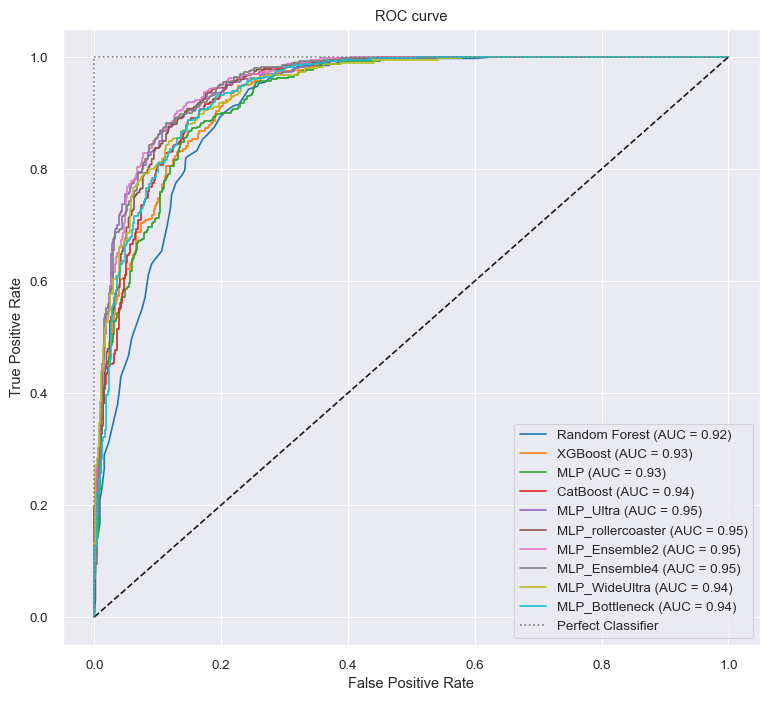
\includegraphics[width=1\columnwidth]{./images/ROC_normVSrest_allmodels.png}
    \caption{ROC curves for the normal class against the rest of the classes across all models.}
    \label{fig:ROC_normVSrest_allmodels}
\end{figure}

To further analyze model performance, we selected four significative FPR levels (1\%, 5\%, 10\%, 20\%) and 
calculated the corresponding TPR. The consolidated results are shown in 
Figure \ref{fig:normVSrest_all}.

\begin{figure*}[htpb]
    \centering
    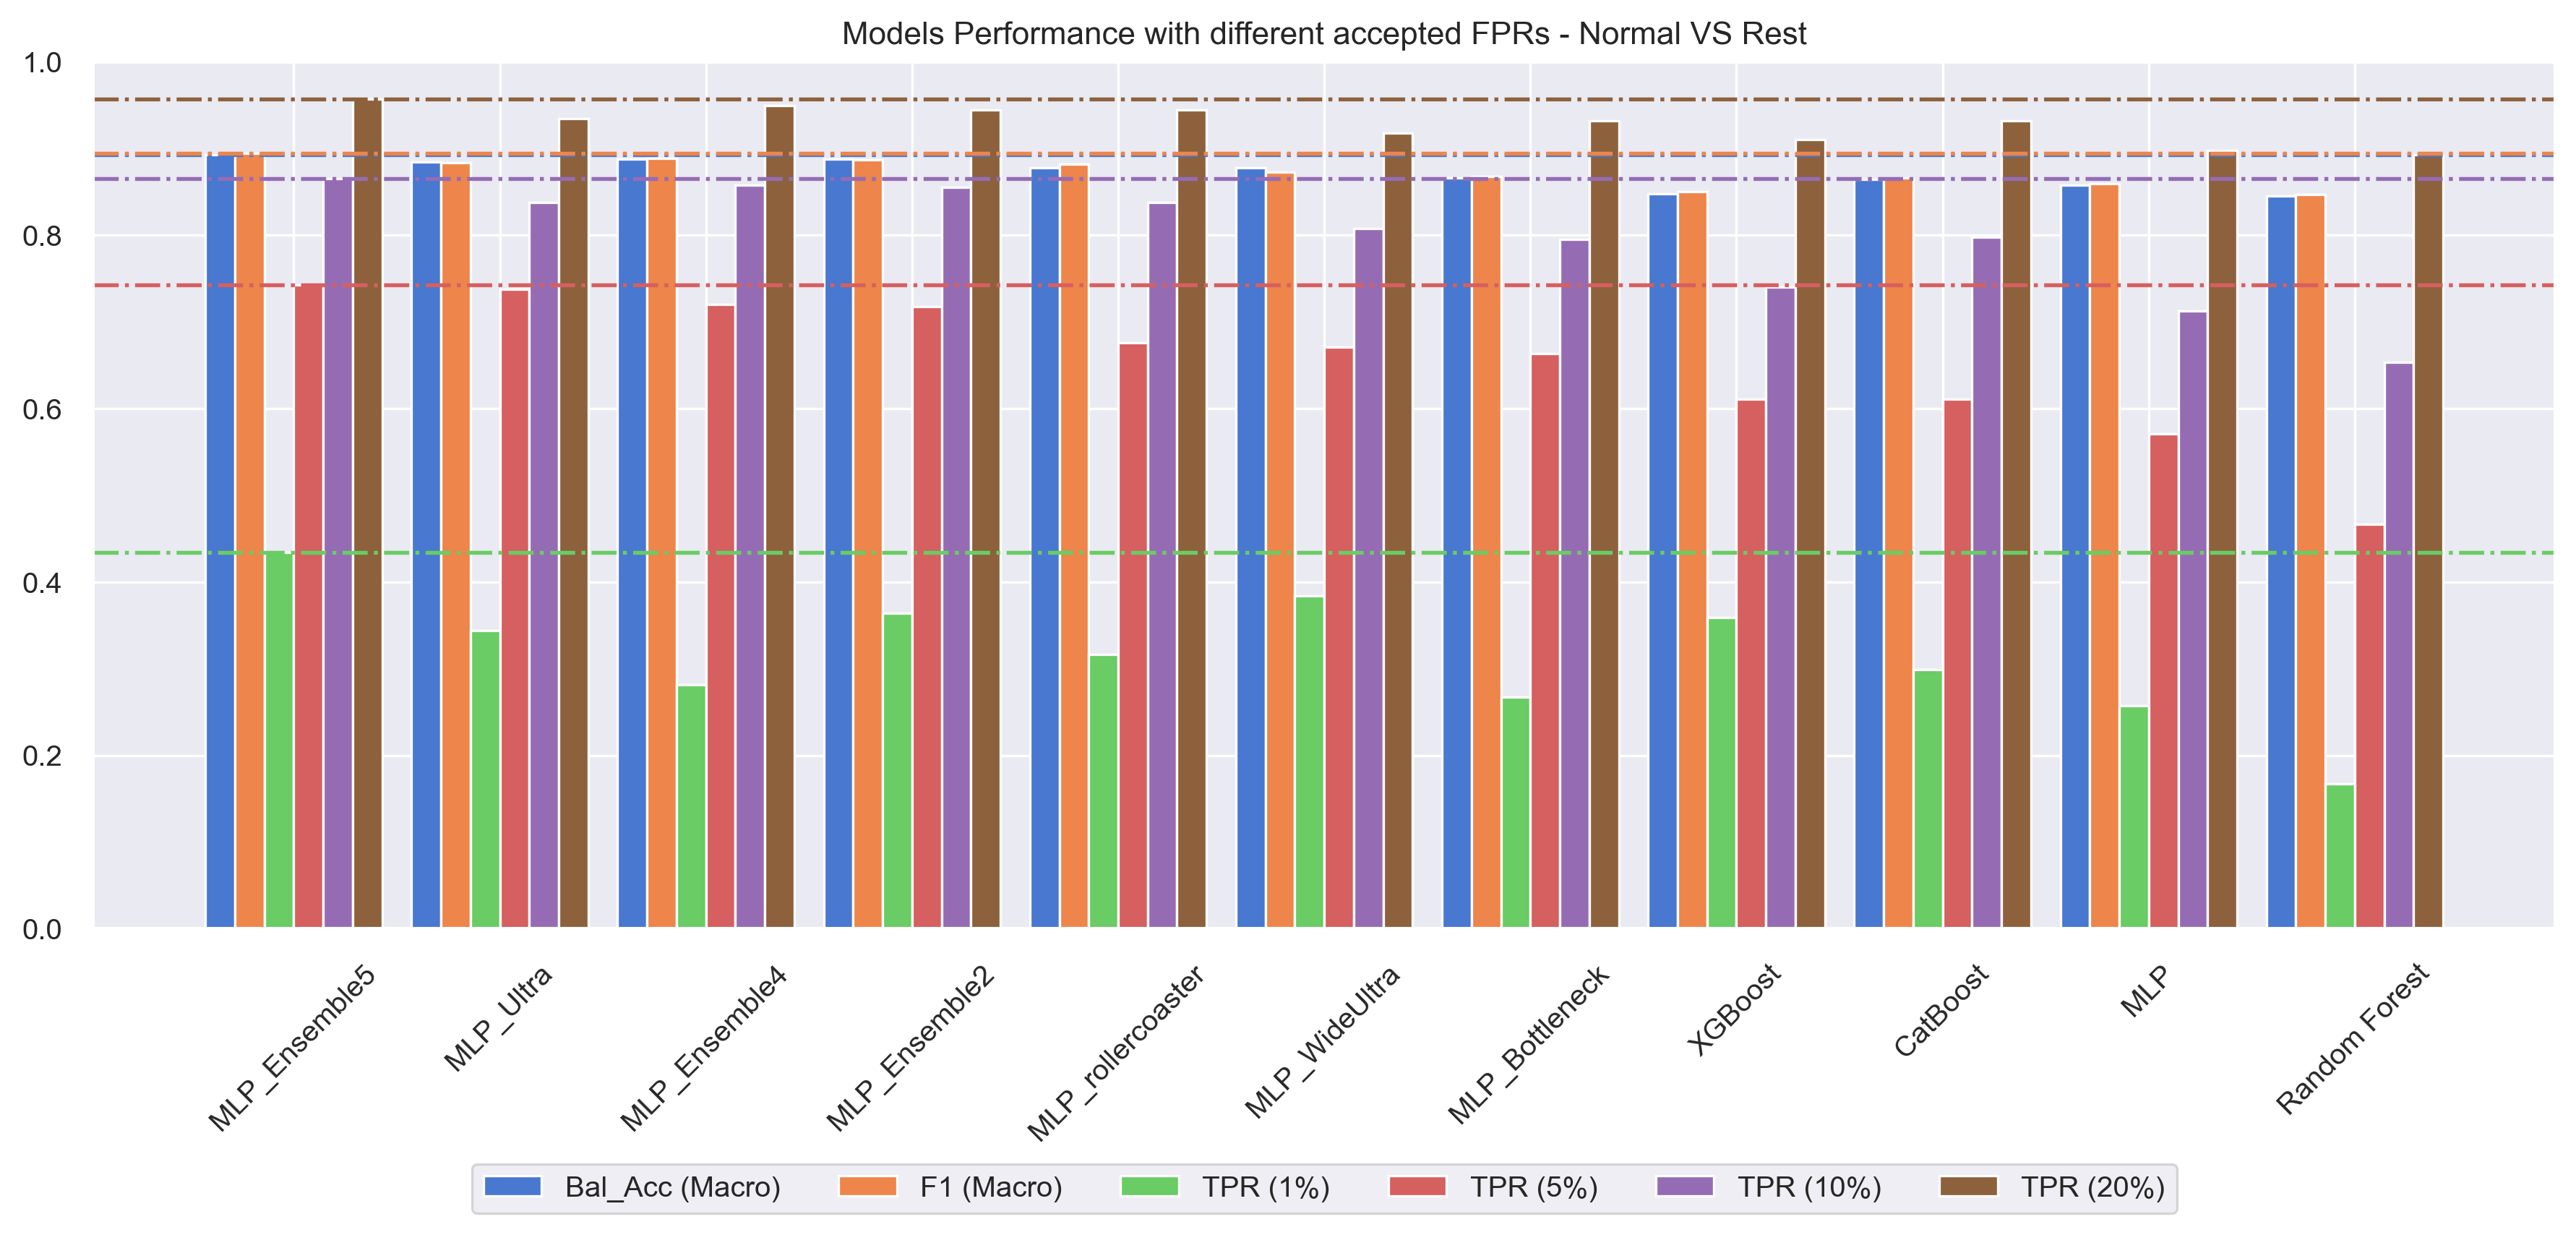
\includegraphics[width=1\textwidth]{./images/nomrVSrest_all.png}
    \caption{TPR at different FPR levels for all models.}
    \label{fig:normVSrest_all}
\end{figure*}

At each FPR level, \textit{MLP\_Ensemble5} outperformed the other models, 
achieving TPRs of 43.4\%, 74.3\%, 86.6\%, and 95.8\% at the 1\%, 5\%, 10\%, and 20\% FPR levels, 
respectively. Excluding \textit{MLP\_Ensemble5}, the best-performing model varied by 
FPR level: \textit{MLP\_WideUltra} at 1\%, \textit{MLP\_Ultra} at 5\%, \textit{MLP\_Ensemble2} at 10\%, 
and \textit{MLP\_Ensemble4} at 20\%.

These outcomes highlight the task's challenges in creating a model that performs well across all FPR 
levels and demonstrate the efficacy of a well-built ensemble model, which leverages the strengths of 
different models to achieve optimal performance.

\subsubsection{Best Model Analysis}
%confmat of the models composing it vs confmat of the ensemble

To understand the performance of the ensemble model (detailed architecture depicted in Figure \ref{fig:MLP_Ensemble5}), we compared its confusion matrix against 
the confusion matrices of the individual models that compose it
(Figure \ref{fig:confmat_ensemble_vs_individual}).

\begin{figure}[H]
    \centering
    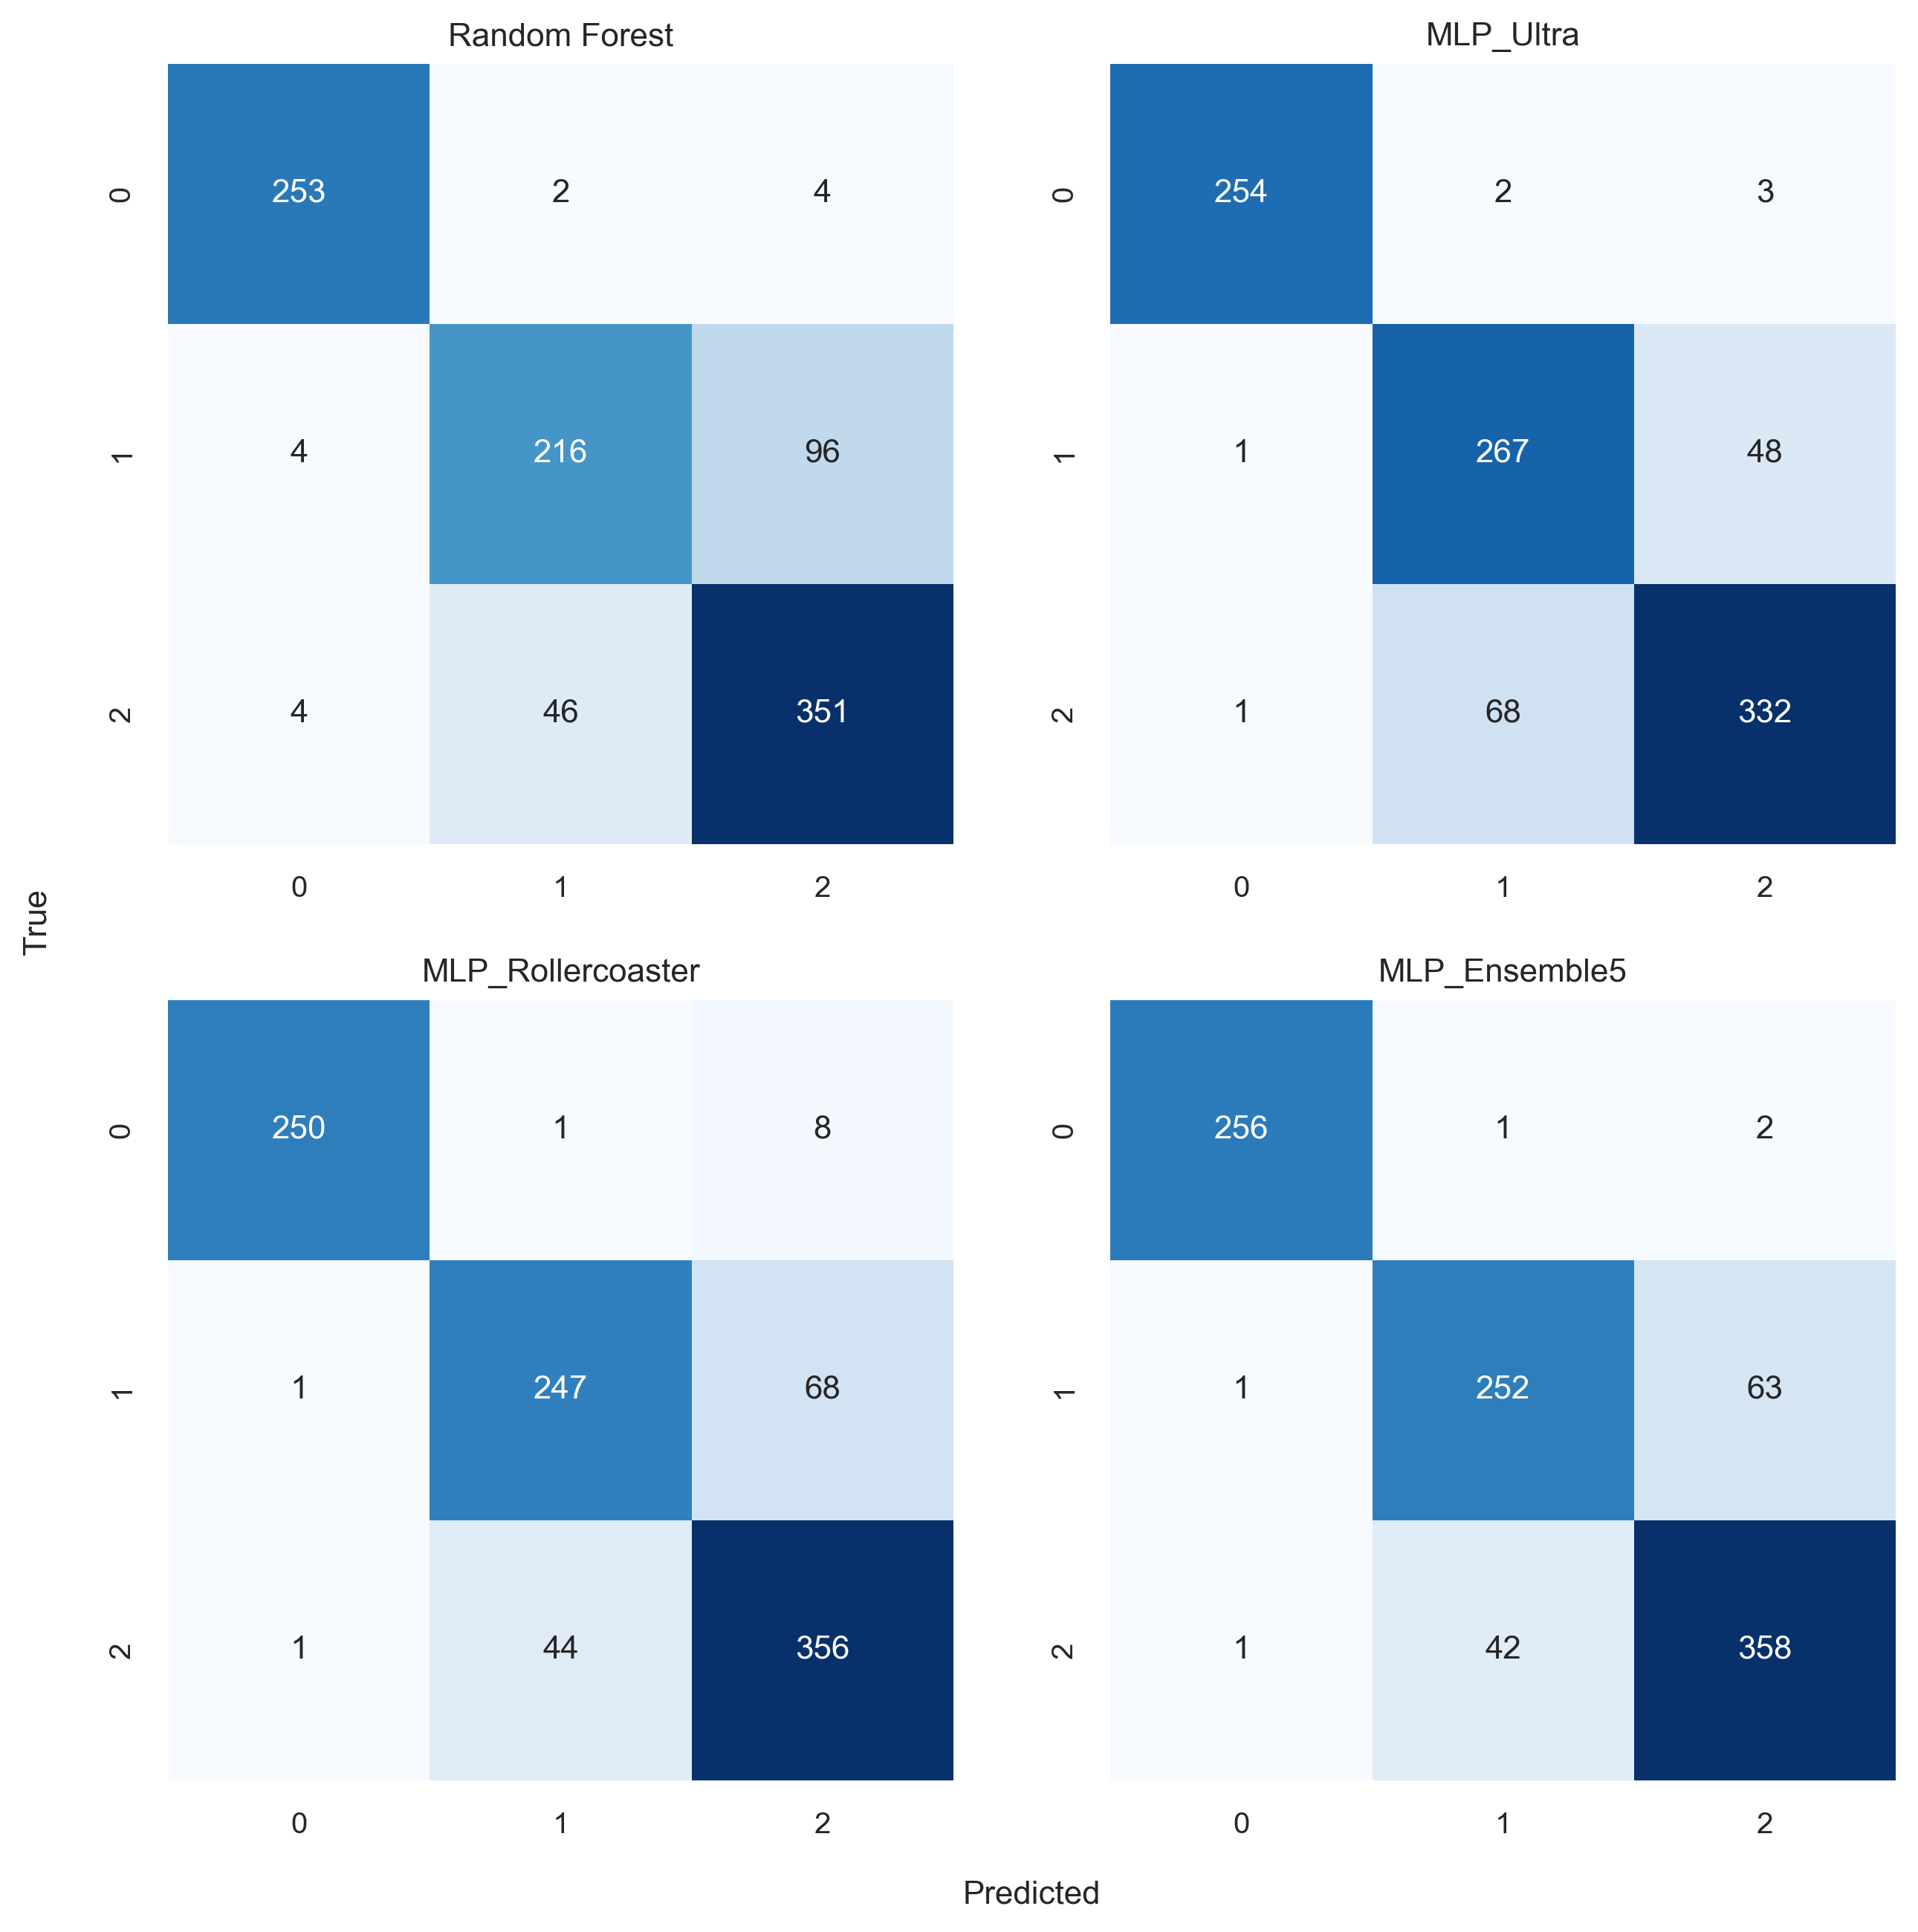
\includegraphics[width=1\columnwidth]{./images/confmat_ensemble_vs_individual.png}
    \caption{Confusion matrices of the individual models and the ensemble model.}
    \label{fig:confmat_ensemble_vs_individual}
\end{figure}

\noindent
In the confusion matrix, class 2 represents normal heartbeats, class 1 represents abnormal heartbeats, and 
class 0 represents artifacts. The Random Forest and MLP\_Ultra models exhibit complementary strengths: the 
Random Forest works better in recognizing normal samples, while the MLP\_Ultra model performs better in 
identifying abnormal samples. The ensemble model effectively combines these strengths.\\\noindent
The contribution of the MLP\_Rollercoaster model to the ensemble’s performance is less apparent but has been 
experimentally demonstrated. This may be due to its ability to correctly classify some samples that are 
misclassified by the other models.\\\noindent
Notably, the MLP\_Ultra model classifies fewer abnormal heartbeats as normal compared to the MLP\_Ensemble5 
model. However, this is because the MLP\_Ultra model simply classifies fewer samples as normal. Minimizing 
the false positive rate (FPR) for the normal class by classifying all samples as abnormal would result in a very 
low true positive rate (TPR) for the normal class. This highlights the importance of analyzing FPR and TPR together.\\\noindent
In conclusion, the ensemble model is the most effective for classifying normal heartbeats, abnormal heartbeats, 
and artifacts, achieving an optimal trade-off between FPR and TPR. % Andrea

\subsection{Support Model}
The support models are evaluated using several metrics, including macro F1 score, accuracy, balanced accuracy, and MCC.
The results are depicted in Figure \ref{fig:support_models_metrics}.\\
From the figure, it is evident that accuracy tends to be higher than other metrics for all models,
indicating a potential bias as it overestimates model performance.\\
Among the models, the MLP ensembles generally show superior performance compared to individual models.
Notably, the MLP\_Ensemble2 model exhibits the highest performance, with a macro F1 score of 81.58 and an MCC of 81.53.
This suggests that ensemble models effectively leverage the strengths of individual models to achieve optimal performance.
\begin{figure}[H]
    \centering
    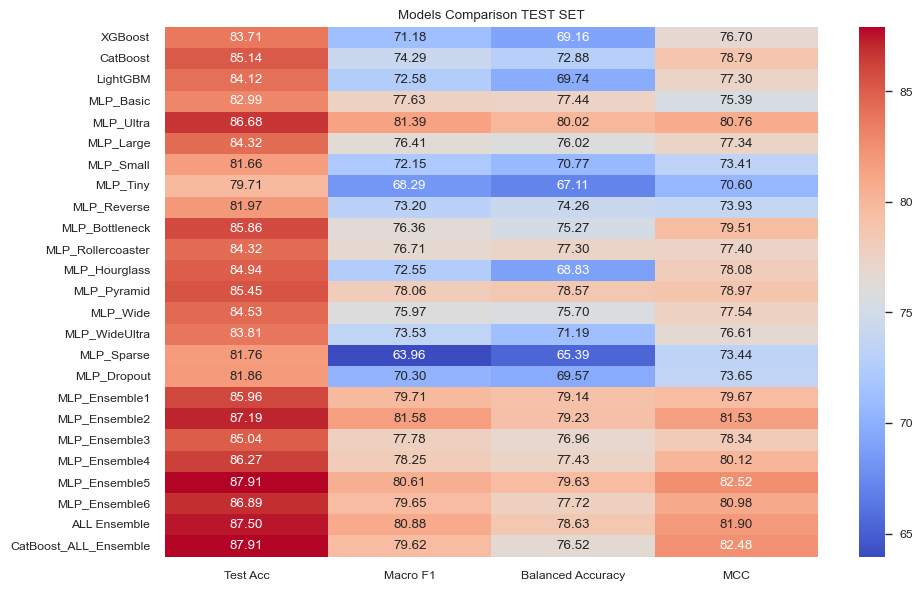
\includegraphics[width=1\columnwidth]{../images/support_models_metrics.png}
    \caption{Metrics of the Support Models, computed on the test set}
    \label{fig:support_models_metrics}
\end{figure}
\noindent
The risk of misclassifying an abnormal sample as normal is depicted in Figure \ref{fig:support_models_risk_scores},
 which shows the overall risk scores (in blue) for each model. The graph also displays specific risk scores associated with each class,
 representing the probability of predicting a sample of that class as normal.\\
This stacked bar chart helps compare the height of the different colors rather than their areas.
 From the figure, it's clear that no single model consistently outperforms others across all scores,but the performance varies across the scores. 
 For instance, MLP\_Rollercoaster has the best overall risk score (blue) and excels in murmurs risk score (red), 
 while MLP\_Ensemble3 performs best for extra systoles risk (orange).

\begin{figure*}[t]
    \centering
    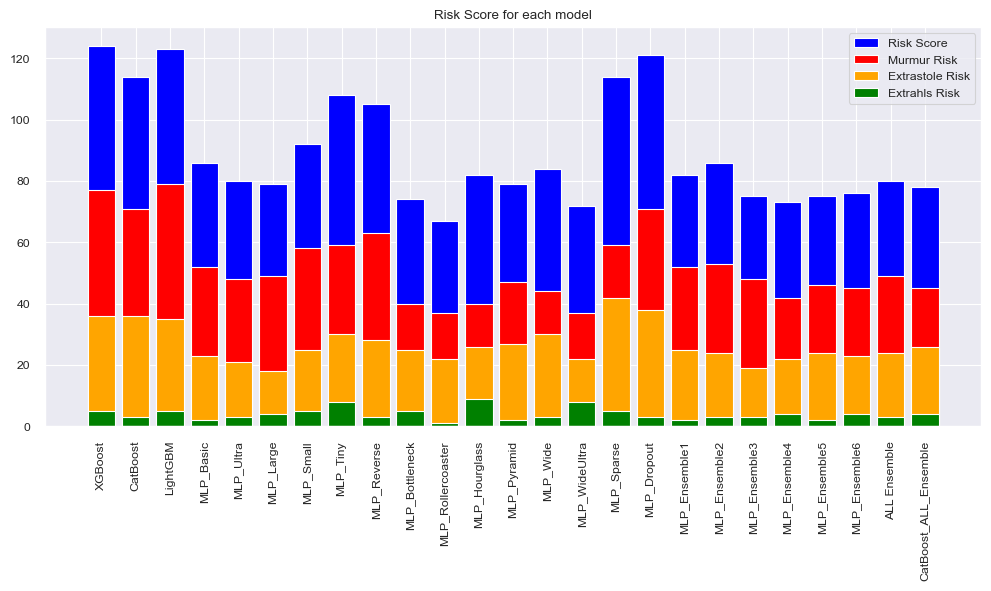
\includegraphics[width=0.8\textwidth]{../images/support_models_risk_scores.png}
    \caption{Risk Scores of the Support Models}
    \label{fig:support_models_risk_scores}
\end{figure*}

\subsubsection*{Best Model}

\begin{figure}[H]
    \centering
    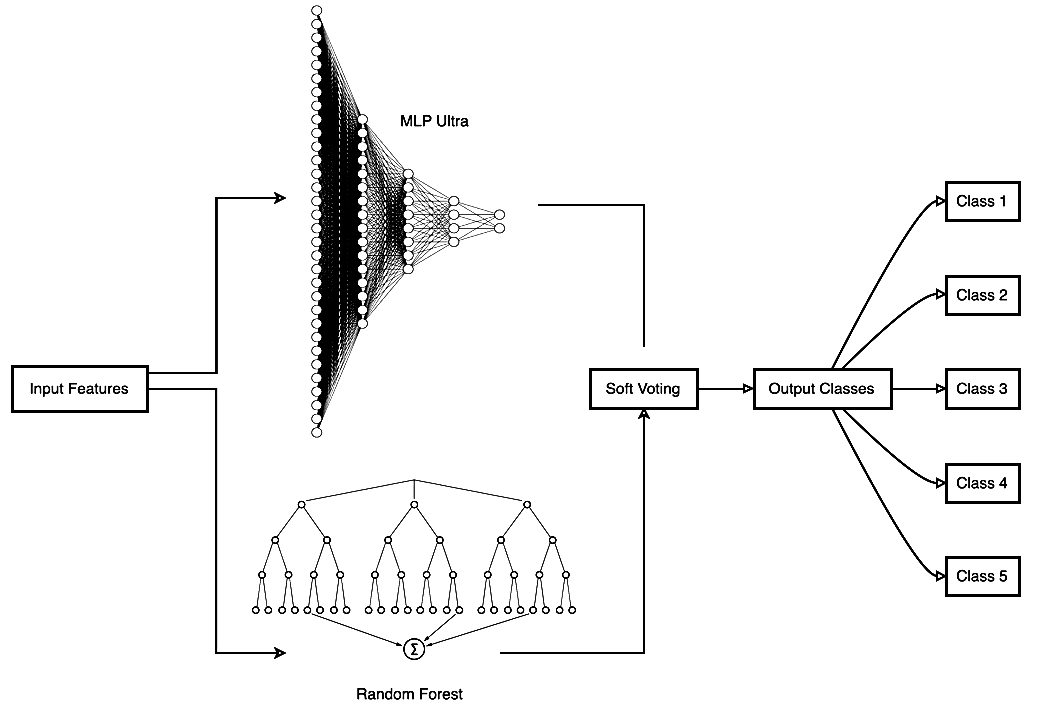
\includegraphics[width=0.8\columnwidth]{../images/MLP_Ensamble2.png}
    \caption{Architecture of the best Support Model}
    \label{fig:MLP_Ensamble2}
\end{figure}
\begin{figure}[H]
    \centering
    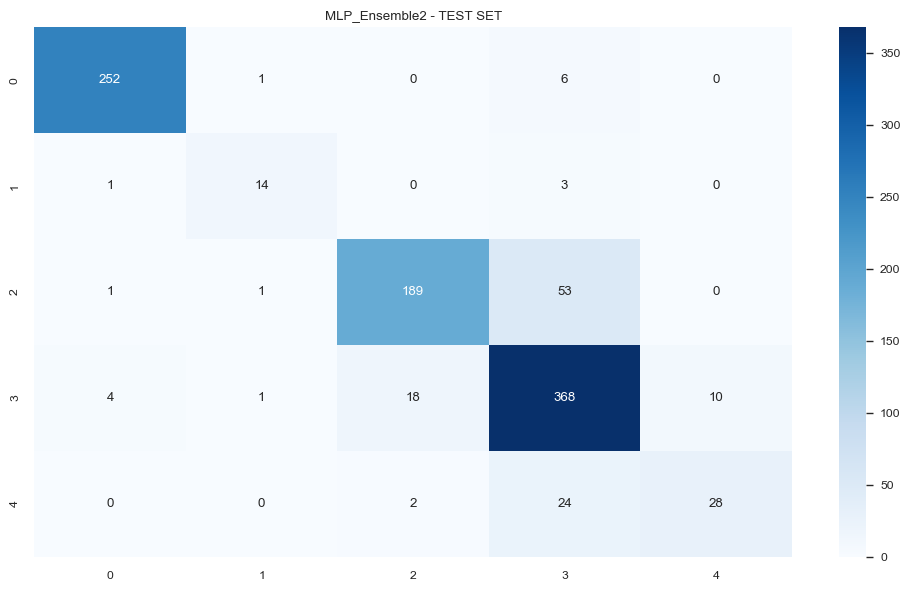
\includegraphics[width=0.8\columnwidth]{../images/support_models_conf_matrix.png}
    \caption{Confusion Matrix of the best Support Model}
    \label{fig:support_models_conf_matrix}
\end{figure}

\begin{figure*}[htpb]
    \centering
    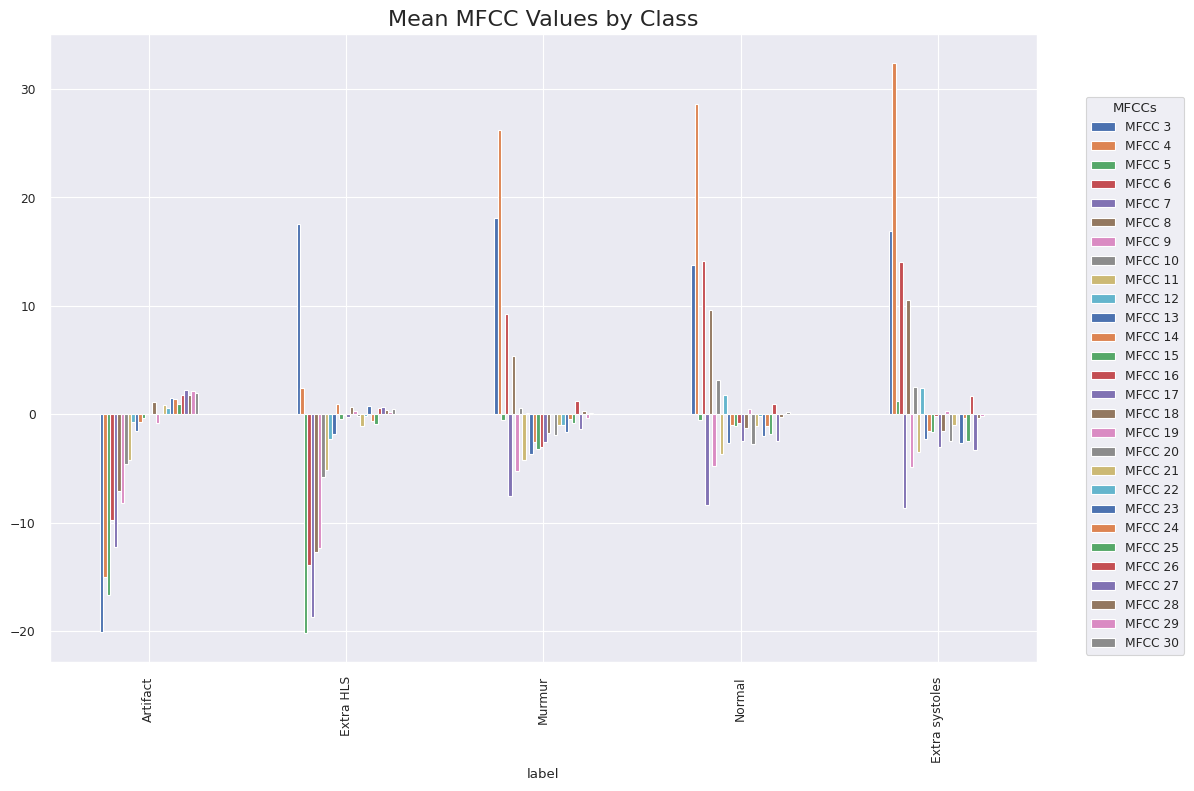
\includegraphics[width=0.8\textwidth]{../images/mean_val_for_features.png}
    \caption{Mean values for each feature within each class}
    \label{fig:mean_val_for_features}
\end{figure*}

\subsubsection*{Explainability}

\begin{figure*}[htpb]
    \centering
    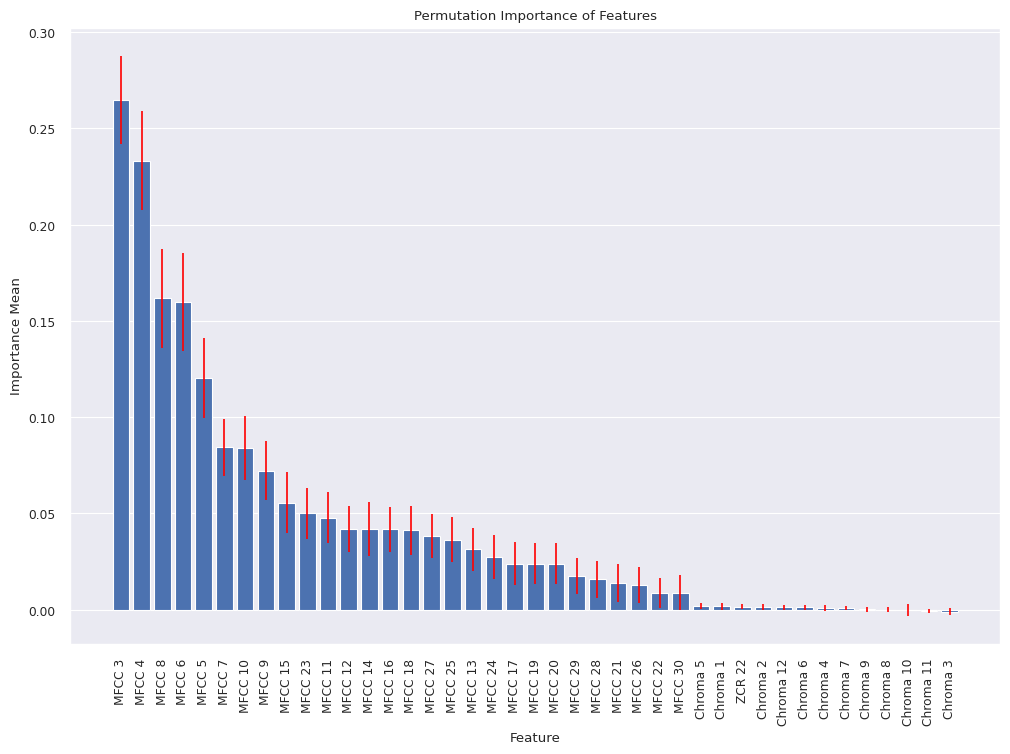
\includegraphics[width=0.8\textwidth]{../images/permutation_feature_importance.png}
    \caption{Feature Importance computed with Permutation Importance}
    \label{fig:permutation_feature_importance}
\end{figure*}


\begin{figure}[H]
    \centering
    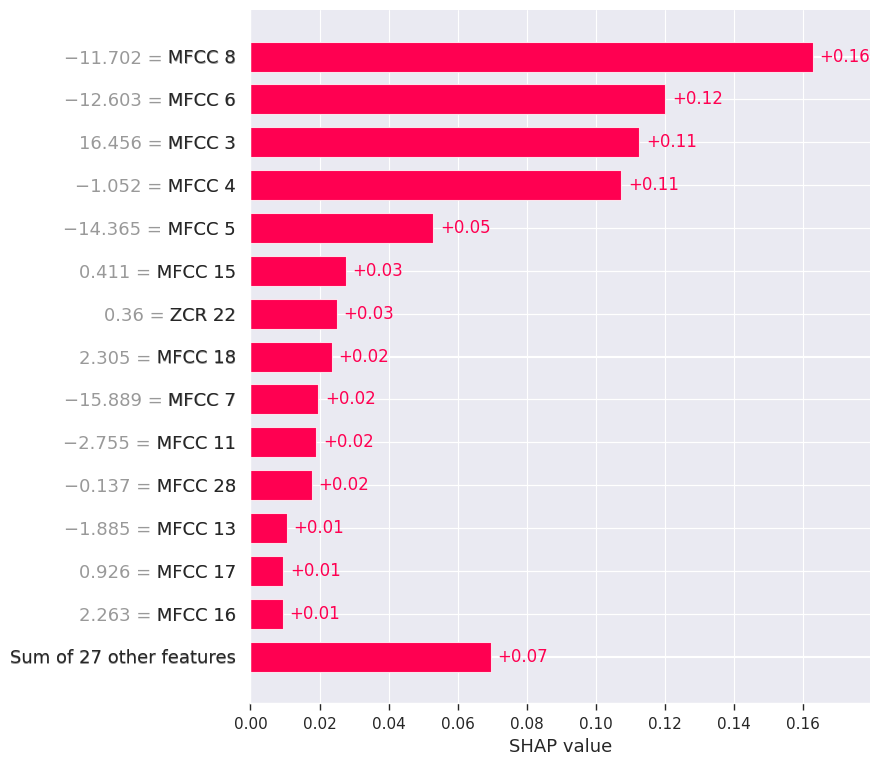
\includegraphics[width=0.8\columnwidth]{../images/extrahls_feature_importance.png}
    \caption{Feature importance for a single extra heart beat sample}
    \label{fig:extrahls_feature_importance}
\end{figure} % Davide

\subsection{Other Experiments}
To further explore the classification problem, we conducted additional experiments 
involving CNN-based feature extraction, data augmentation, and a novel approach 
using a tiered ensemble model.

\subsubsection*{CNN-Based Experiments}

We conducted a series of experiments using Convolutional Neural Networks (CNNs) to explore their 
effectiveness as feature extractors for the 5-class classification problem. The CNN was
used with ImageNet weights and was not fine-tuned.

\begin{itemize}[leftmargin=*]
    \item \textbf{VGG16 with Spectral Features}: VGG16 CNN was employed as a feature extractor with 
    spectral features (MFCC, CQT, Chroma STFT, among others) used as input images. This approach yielded 
    a Macro F1 score of approximately 65\%, which is lower than the performance achieved in the primary 
    work.
    \item \textbf{VGG16 with Raw Waveform Images}: VGG16 was also used to extract features from raw 
    waveform images. Features were taken from the 5th, 4th, and 3rd convolutional layers after pooling, 
    and various classifiers (RF, SVM, MLP) were tested on these features. This method resulted in a 
    performance of around 67\%.
\end{itemize}

\subsubsection*{Data Augmentation}
\label{sec:data_augmentation}

We explored data augmentation techniques to address the limited and imbalanced dataset and improve
the model's generalization capabilities.

\begin{itemize}[leftmargin=*]
    \item \textbf{Noise Addition and Speed/Pitch Alteration}: We augmented the data by adding random noise (factor 0.05)
    and altering speed and pitch. However, the improvement in performance was not significant. 
    This may be due to the limited size and inherent imbalance of the dataset, as data augmentation 
    did not alter the class distribution.
    \item \textbf{Synthetic Data Generation with SMOTEN}: Synthetic data generation was applied to the 
    less represented classes using SMOTEN. Although there was an initial spike in performance metrics, 
    this was identified as bias. The model could easily distinguish the synthetically generated data from 
    the original data. The underlying issue was the limited size of the original dataset, which did not 
    provide sufficient variability for the synthetic generation algorithm to produce realistic 
    and diverse samples.
\end{itemize}

\subsubsection*{Tiered Ensemble Model}

We attempted to decompose the classification problem into two sub-problems, according to Figure \ref{fig:tiered_ensemble}.

\begin{itemize}[leftmargin=*]
    \item \textbf{Sub-problem 1: Artifact, Normal, and Abnormal Classification}: Various models were 
    tested for distinguishing between artifact, normal, and abnormal audio. The best model 
    (MLP\_Ensemble5) achieved a balanced accuracy of approximately 89.2\%.
    \item \textbf{Sub-problem 2: Disease Classification}: Different models were also applied to 
    distinguish between different diseases, achieving a balanced accuracy of more than 90.3\% with MLP\_Ensemble2.
    \item \textbf{Final Ensemble Model}: A third model (CatBoost) was used to integrate the predictions 
    from the above sub-problems and make the final classification among the five classes. This ensemble 
    approach resulted in a balanced accuracy of 80.5\%.
\end{itemize}

\begin{figure}[H]
    \centering
    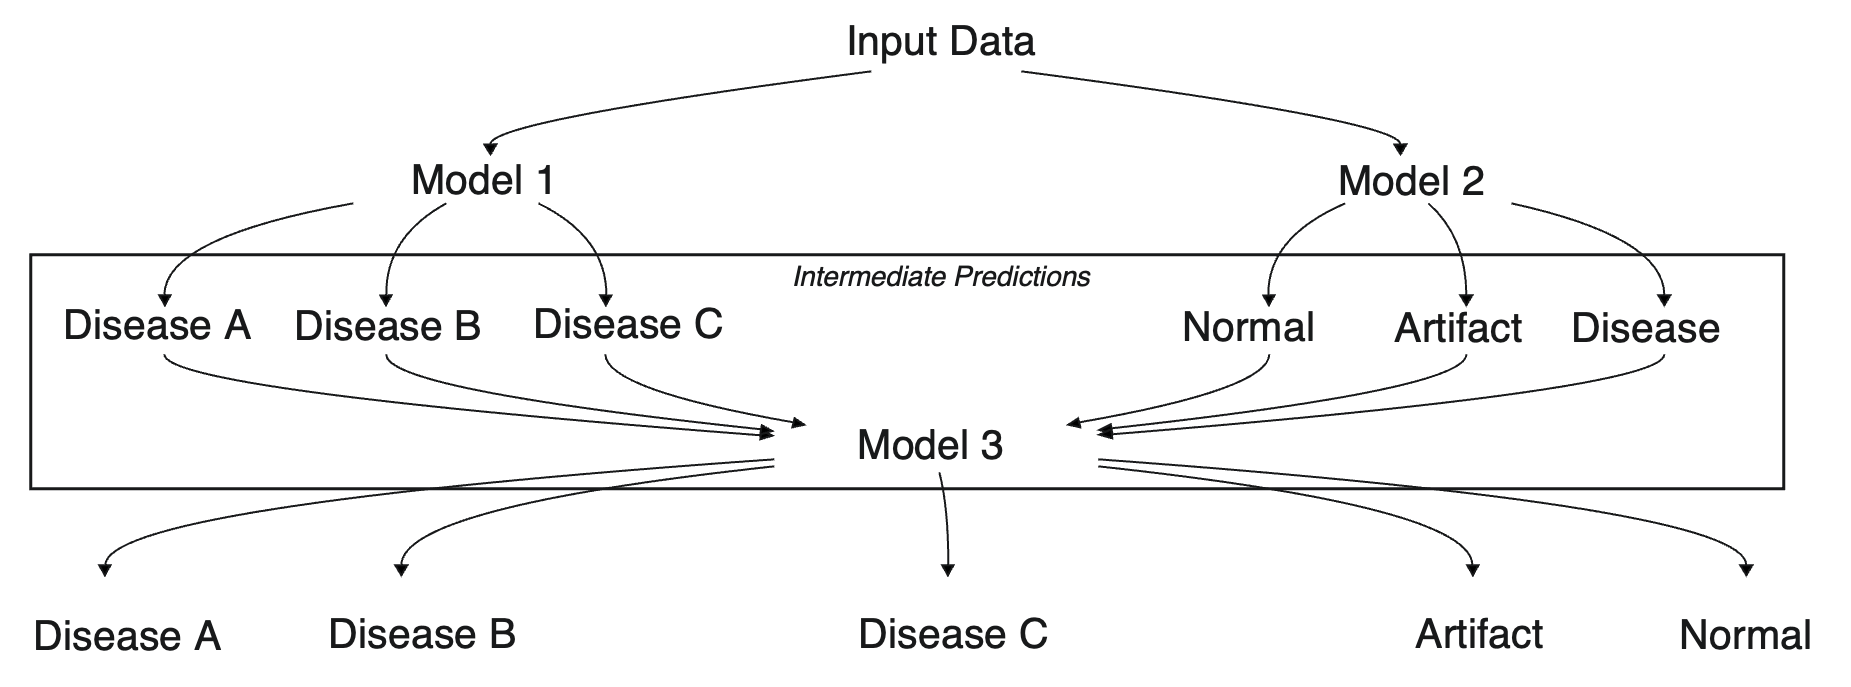
\includegraphics[width=1\columnwidth]{images/tiered_ensemble.png}
    \caption{Tiered Ensemble Model}
    \label{fig:tiered_ensemble}
\end{figure}

\noindent
Despite the promising results, the tiered ensemble model did not outperform the primary models.
 % Andrea

% Section discussion
\section{Discussion}

In our research, we developed two ensemble models, MLP\_Ensemble5 and MLP\_Ensemble2, to address the dual purpose of enhancing prevention and diagnosis
(support model) of heart disease. For MLP\_Ensemble5, our focus was on minimizing false normals, ensuring that potential heart diseases are not overlooked.
On the other hand, MLP\_Ensemble2 aimed to maximize overall predictive performance while incorporating explainability
to provide valuable insights to medical professionals.\\
Our experimentation involved various models and features, with careful consideration of correlation aspects,
to achieve the best results. We utilized the PASCAL challenge dataset and addressed the class imbalance problem by aggregating diseases
in one instance and employing appropriate metrics in another.\\
Several studies have explored heart disease prediction using machine learning. Zhang et al. \cite{Zhang_Han_Deng_2017}
utilized a Support Vector Machine (SVM) model with spectrogram features, achieving a precision of 0.76, while Deng et al. \cite{Deng_Han_2016}
used SVM with Discrete Wavelet Transform (DWT) features, obtaining similar precision.
Although these models are computationally efficient, their performance is limited.
Advancements in deep learning, such as the Long Short-Term Memory (LSTM) model used by Raza et al. \cite{Raza_Mehmood_Ullah_Ahmad_Choi_On_2019}
with 1D time series features, achieved an accuracy of 0.80 with Normal, Murmur, and Extrasystole classes.\\
Significant improvements in accuracy were achieved using Convolutional Neural Networks (CNNs)
by Alafif et al. \cite{Alafif_Boulares_Barnawi_Alafif_Althobaiti_Alferaidi_2020} and Noman et al. \cite{Noman_Ting_Salleh_Ombao_2019},
although they only considered Normal and Abnormal classes. A more disease-specific approach was taken
by Chen et al. \cite{Chen_Ren_Hao_Hu_2018}, who used a 2D CNN model with Wavelet Transform and Hilbert-Huang features, achieving an
accuracy of 0.93 with Normal, Murmur, and Extrasystole classes. This high accuracy highlights the potential for
improving our support model, which struggles to distinguish between Murmur, Normal, and Extrasystole classes.\\
Direct comparisons between studies are challenging due to differences in datasets and class definitions.
Our model uniquely considers five classes, making it distinct from others. Furthermore, the choice of evaluation metrics is crucial when dealing
with imbalanced datasets, as accuracy can be misleading.\\
Our research contributes to the literature by presenting two models. MLP\_Ensemble5 was optimized to minimize
false normals while maintaining low computational costs and distinguishing between disease presence and artifact signals.
MLP\_Ensemble2 was optimized for overall performance and introduced explainability measures to assist medical staff.\\
Despite these advancements, our project faced limitations. The limited dataset size prevented the creation of a validation set, potentially biasing results.
Additionally, to increase data availability, we selected a one-second extraction interval, which may not be optimal due to varying heart rates.
This approach might result in samples lacking relevant information if the full cardiac cycle is not present within the interval.\\
Feature selection also posed challenges. While MFCCs proved effective, they were not sufficiently discriminative for distinguishing between Normal,
Murmur, and Extrasystole classes, where our model struggled the most. Furthermore, the explainability of the model has its constraints.
We identified significant temporal regions on the waveform based on MFCC values within these regions. 
According to SHAP values, these specific MFCC values help to classify the sample correctly.
 However, the model only understands the average temporal values, not the instantaneous ones. 
 Consequently, the explanation provided by the model is limited and requires further validation to be considered reliable.\\
Finally, the representativeness of the dataset remains a major obstacle to developing a model suitable for real-world scenarios.
Addressing these limitations in future research could enhance the applicability and reliability of our models in clinical settings.


% Section Conclusion
\section{Conclusion}
\subsection{Overall Impression}

\subsection{Future Work}

\clearpage
\section{Appendix}

% Figure on the best prevention model


% color the image in black
\begin{figure}[H]
    \centering
    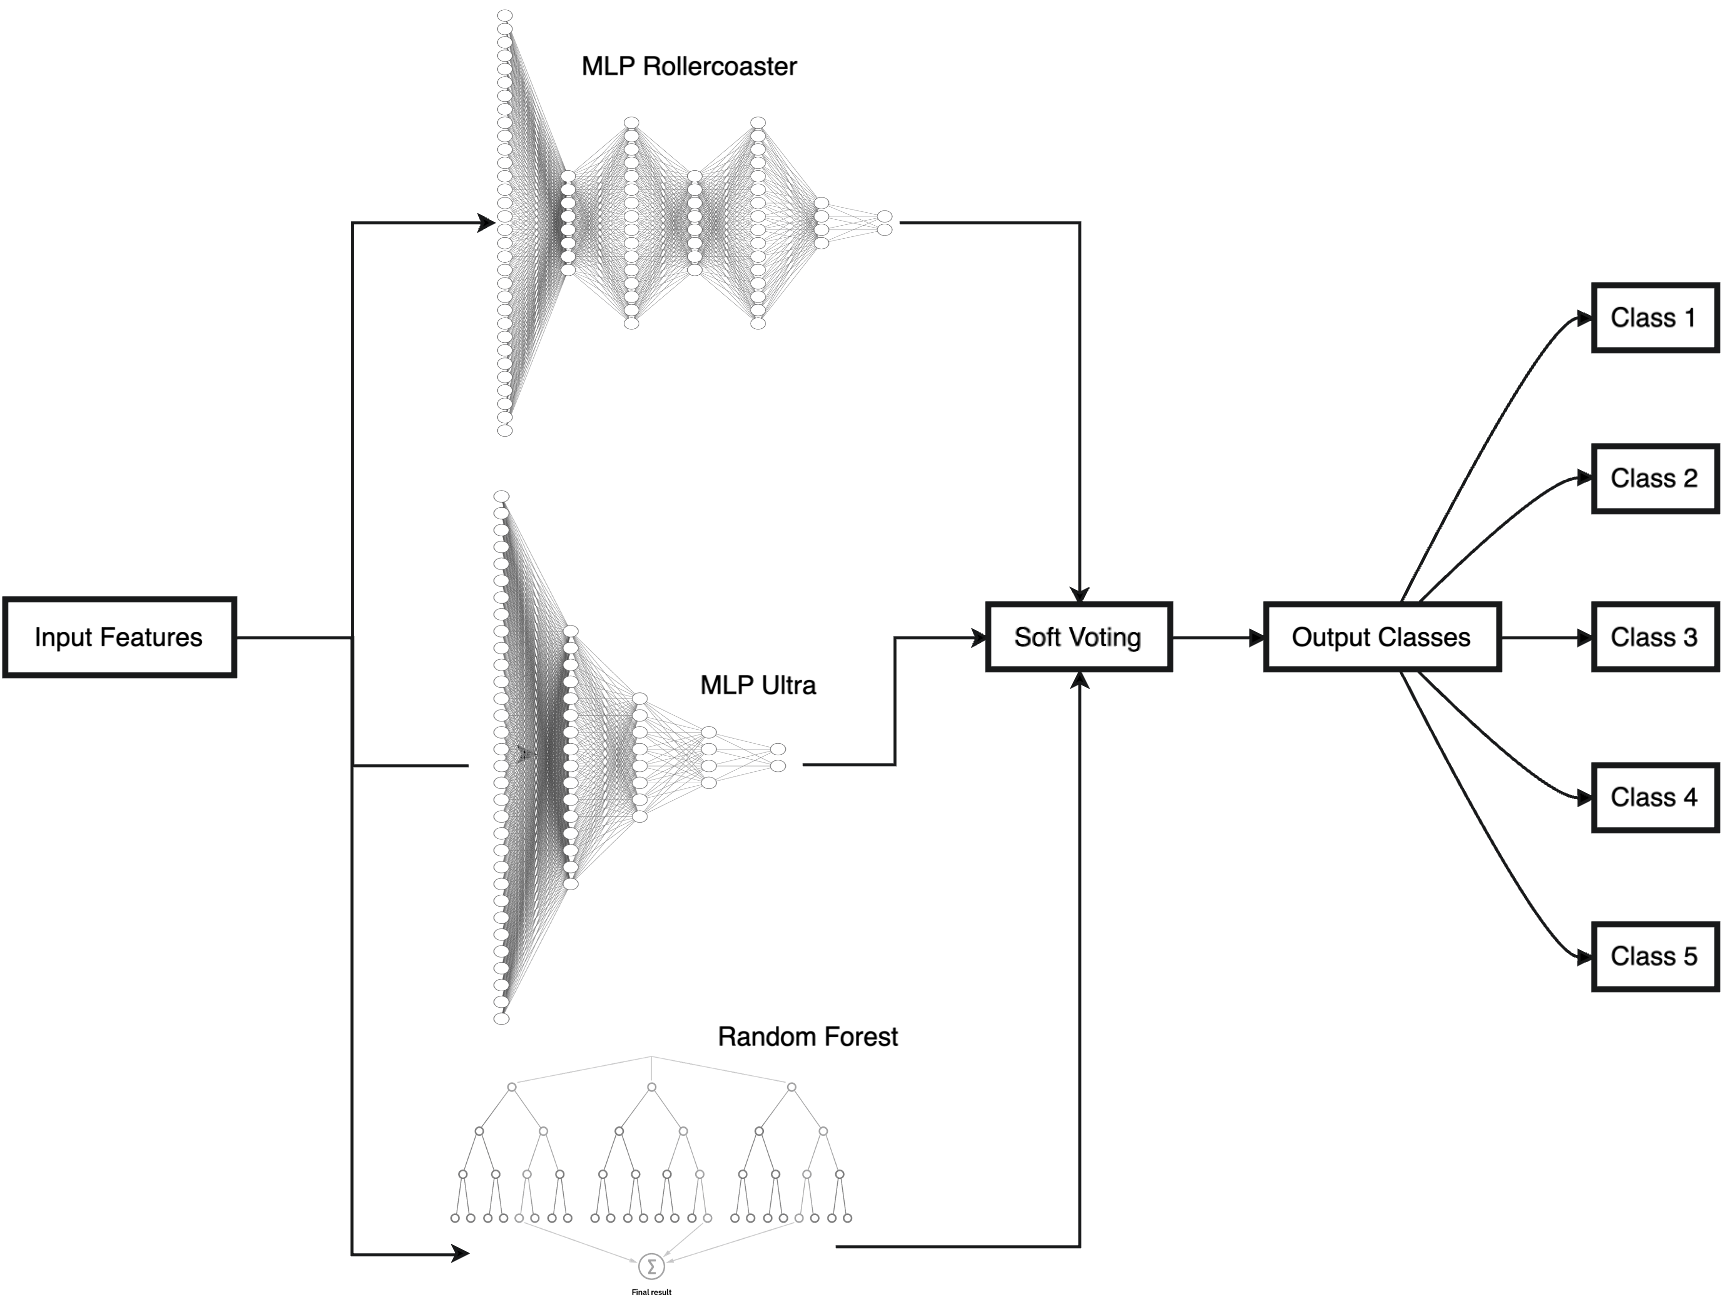
\includegraphics[width=1\columnwidth]{./images/MLP_Ensemble5.png}
    \caption{MLP Ensemble5 Architecture}
    \label{fig:MLP_Ensemble5}
\end{figure}

\clearpage
\printbibliography

\end{document}